\documentclass[11pt]{article}

\usepackage[margin=1in]{geometry}
\usepackage{graphicx}
\usepackage{amsmath,amssymb}
\usepackage{booktabs}
\usepackage{hyperref}
\usepackage{xcolor}
\usepackage{caption}
\usepackage{subcaption}
\usepackage{microtype}

\hypersetup{colorlinks=true, linkcolor=blue, citecolor=blue, urlcolor=blue}

\title{Learning Conway's Game of Life with CNN-Transformer Hybrids:\\
Architecture Scaling, Exposure Bias, and Activation Inductive Bias}
\author{Hao-Yuan}
\date{\today}

\begin{document}

\maketitle

\begin{abstract}
We study the problem of learning the one-step transition rule of Conway's
Game of Life (GoL) on a $40\times40$ toroidal grid using a CNN-Transformer
hybrid architecture. Starting from a model trained with pure teacher forcing,
we show that autoregressive rollout suffers from exposure bias: the model
diverges on sparse configurations it never sees during single-step training.
We show that a straight-through-estimator (STE) multi-step training scheme
fails due to a systematic gradient bias, while scheduled sampling resolves
the issue cleanly. We further show that once a $291$K-parameter model
saturates its representational capacity, scaling the training set five-fold
\emph{regresses} performance, while scaling the model five-fold to $1.5$M
parameters eliminates essentially all remaining errors. Motivated by recent
work on activation-function inductive bias for cellular automata
(Ahmed \& Davis, 2026), we independently reproduce their central finding
that a learnable second-degree polynomial activation lets a $25$--$34$
parameter CNN learn GoL reliably where ReLU fails almost completely, and we
report a negative result from attempting to transfer this activation into
our larger multi-step model. Finally, we analyze the learned patch
embeddings of our best models under geometric transformations and cellular
perturbations, characterizing how content, absolute position, and
attention-mediated context interact in the representation space.
\end{abstract}

\tableofcontents

\section{Introduction}

Conway's Game of Life (GoL) is a deterministic cellular automaton defined on
a two-dimensional grid, where each cell is alive or dead and updates
synchronously according to a fixed local rule (B3/S23): a dead cell with
exactly 3 live neighbors becomes alive (\emph{birth}); a live cell with 2 or
3 live neighbors stays alive (\emph{survival}); all other cells die or
remain dead. Despite the simplicity of the rule, GoL exhibits rich emergent
dynamics (oscillators, spaceships, and chaotic regimes at high density),
which makes it a useful and cheaply-simulated testbed for studying whether
neural networks can learn a precisely-specified local update rule from
examples, and how architectural and training choices affect that learning.

This report documents an iterative series of experiments training a
CNN-Transformer hybrid to predict one GoL step ahead on a $40\times 40$
toroidal (periodic-boundary) grid. The narrative proceeds through three
largely independent threads:

\begin{enumerate}
  \item \textbf{Training dynamics for multi-step prediction}
  (Section~\ref{sec:training-evolution}). A model trained purely with
  teacher forcing (always conditioning on the ground-truth previous frame)
  performs well on single-step prediction but collapses under its own
  autoregressive rollout, particularly on sparse configurations. We compare
  a straight-through-estimator (STE) approach to multi-step training against
  scheduled sampling, and show that only the latter is stable.

  \item \textbf{Model capacity vs.\ data scale}
  (Section~\ref{sec:results-table}). Once a model of a given size is
  performing near-perfectly on average, we show that increasing the
  \emph{training set size} five-fold can \emph{regress} accuracy on hard
  (high-density) grids, while increasing \emph{model capacity} five-fold
  removes essentially all remaining errors. This is consistent with the
  model having saturated its representational capacity rather than being
  data-limited.

  \item \textbf{Activation-function inductive bias}
  (Section~\ref{sec:verification}). Motivated by a recent paper on
  Kolmogorov-Arnold-style polynomial activations for GoL
  \cite{ahmed2026polynomial}, we independently reproduce its central claim
  on our own $40\times 40$ toroidal setup using an from-scratch
  reimplementation of their minimal architecture, and separately report a
  negative result from attempting to transfer the same activation into our
  larger multi-step CNN-Transformer.
\end{enumerate}

Section~\ref{sec:architecture} describes the shared CNN-Transformer
architecture used throughout. Section~\ref{sec:embedding-analysis} presents
an interpretability study of the learned patch embeddings under geometric
transformations (rotation, reflection, translation) and local perturbations
(single-cell flips and moves), aimed at understanding how content,
positional encoding, and attention-mediated context jointly determine the
representation of a grid patch.

\section{Architecture}
\label{sec:architecture}

All models in Sections~\ref{sec:training-evolution}--\ref{sec:embedding-analysis}
share the same \emph{CNN-Transformer} architecture (referred to as
\texttt{CNNTransformerV4} in the codebase), operating on a $40 \times 40$
binary grid with toroidal (periodic) boundary conditions. The forward pass
has three stages:

\paragraph{Stage 1 --- Local CNN feature extractor.}
Two $3\times 3$ convolutions with \texttt{circular} padding mode (so that
convolution respects the toroidal topology exactly, rather than treating
the grid border as a hard edge), each followed by GroupNorm and a GELU
nonlinearity:
\[
  \text{Conv2d}(1 \to 32) \to \text{GroupNorm} \to \text{GELU}
  \to \text{Conv2d}(32 \to d_{\text{model}}) \to \text{GroupNorm} \to \text{GELU}.
\]
The receptive field of this stage is $5\times 5$, matching (and slightly
exceeding) the Moore neighborhood relevant to the GoL update rule.

\paragraph{Stage 2 --- Patch tokenization.}
The $40\times 40$ feature map is partitioned into non-overlapping
$4\times 4$ patches (a $10\times 10$ arrangement, $100$ patches total),
following the patch-tokenization scheme of Vision Transformers
\cite{dosovitskiy2020vit}. Each
patch's $d_{\text{model}} \times 4 \times 4$ feature block is flattened and
linearly projected to a $d_{\text{model}}$-dimensional token, and a
\emph{learnable} absolute positional embedding
$\texttt{pos\_embed} \in \mathbb{R}^{100 \times d_{\text{model}}}$ is added:
\[
  \text{token}_i = \text{Linear}(\text{feat}_i) + \text{pos\_embed}_i,
  \qquad i = 1, \dots, 100.
\]
We refer to this as the \textbf{pre-transformer embedding} in
Section~\ref{sec:embedding-analysis}.

\paragraph{Stage 3 --- Transformer encoder.}
A pre-norm Transformer encoder \cite{vaswani2017attention} (GELU
activation, $\text{dim\_feedforward} = 4 d_{\text{model}}$) mixes
information across all 100 patch tokens via
self-attention. We refer to its output as the \textbf{post-transformer
embedding}. A final linear head maps each output token back to
$4\times 4 = 16$ logits, reconstructing next-state predictions for every
cell in the patch.

\paragraph{Model sizes used.} Two sizes appear throughout this report:

\begin{center}
\begin{tabular}{lccccc}
\toprule
Name & $d_{\text{model}}$ & heads & layers & dim\_feedforward & params \\
\midrule
V8 (baseline size)  & 64  & 4 & 4 & 256 & 291{,}888 \\
V10 (scaled size)   & 128 & 8 & 6 & 512 & 1{,}504{,}240 \\
\bottomrule
\end{tabular}
\end{center}

\paragraph{Data augmentation.} Training uses the dihedral group $D_4$
(90$^\circ$ rotations and horizontal/vertical reflections) applied jointly
to input and target frames. Translation augmentation is deliberately
\emph{not} used, since it directly conflicts with the learnable absolute
positional embedding in Stage 2 (a translated patch would need a different
position embedding than the one it is assigned).

\section{Training Dynamics for Multi-Step Prediction}
\label{sec:training-evolution}

\subsection{Baseline: single-step teacher forcing (V5)}

The V5 model is trained with plain single-step supervision: at every
optimization step, the model observes the ground-truth frame at time $t$
and is trained (binary cross-entropy with label smoothing $\varepsilon=0.1$)
to predict the ground-truth frame at $t+1$. This is standard \emph{teacher
forcing} and never exposes the model to its own prediction errors during
training.

V5 reaches strong single-step metrics (best validation loss $0.20125$,
precision $99.4\%$, recall $99.7\%$), but per-event accuracy reveals a
weakness: \emph{born} accuracy (correctly predicting a birth, i.e.\
dead$\to$alive) is only $93.8\%$, well below \emph{survival} accuracy
($99.8\%$) and \emph{death} accuracy ($99.9\%$). When the trained model is
unrolled autoregressively (feeding its own prediction back in as the next
input, rather than the ground truth), sparse configurations tend to
collapse to the all-dead state after a handful of steps: because the model
was never trained on grids containing its own error patterns, occasional
missed births are never corrected and instead compound, until the local
neighborhood has too few live cells to sustain any further births. This is
the classic \emph{exposure bias} problem for autoregressive sequence models.

\begin{figure}[htbp]
  \centering
  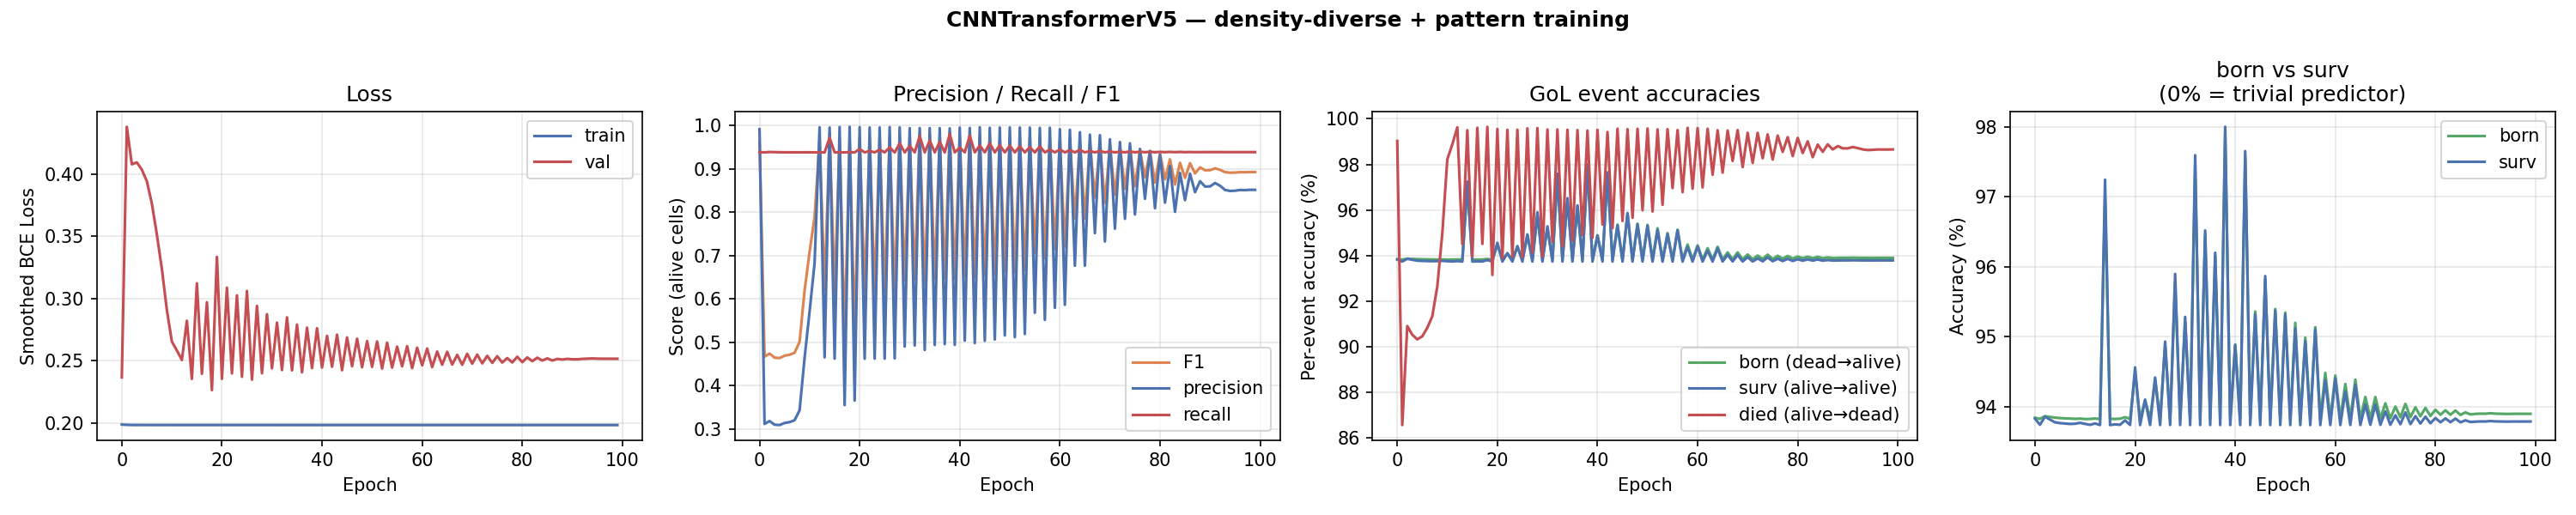
\includegraphics[width=0.85\textwidth]{figures/v5_loss.png}
  \caption{V5 training curves (single-step teacher forcing). Aggregate
  metrics look strong, but this model still collapses under
  autoregressive rollout on sparse grids.}
  \label{fig:v5-loss}
\end{figure}

\subsection{Failed fix: straight-through estimator multi-step training (V6)}

To directly train for rollout stability, V6 unrolls the model for $K=3$
steps during training. At each step, the model's \emph{hard} (binarized)
prediction is fed forward as the next input, while gradients are passed
back through the \emph{soft} (sigmoid) prediction via a straight-through
estimator (STE) --- i.e., $\text{forward} = \mathbb{1}[\sigma(x) > 0.5]$,
$\text{backward} = \nabla \sigma(x)$.

V6 performs well only transiently: at epoch 5 (warm-started from V5) it
reaches validation loss $0.23421$ with precision $92.7\%$ and born-accuracy
$99.5\%$, but precision then collapses to $20$--$50\%$ over the following
epochs and oscillates chaotically through epoch 50 (Figure~\ref{fig:v6-loss}).
Gradient clipping (already active at $\text{max\_norm}=1.0$) does not
resolve this. We hypothesize the failure mode is a \emph{systematic
directional gradient bias}: when the model misses a birth at step $t$, step
$t+1$'s input is missing a live cell relative to ground truth, and the STE
gradient at step $t+1$ consistently signals ``predict more alive'' back
through the network, regardless of whether more alive cells are actually
correct at $t$. This creates a positive-feedback loop toward over-predicting
liveness that is not a magnitude problem (which clipping could fix) but a
\emph{direction} problem.

\begin{figure}[htbp]
  \centering
  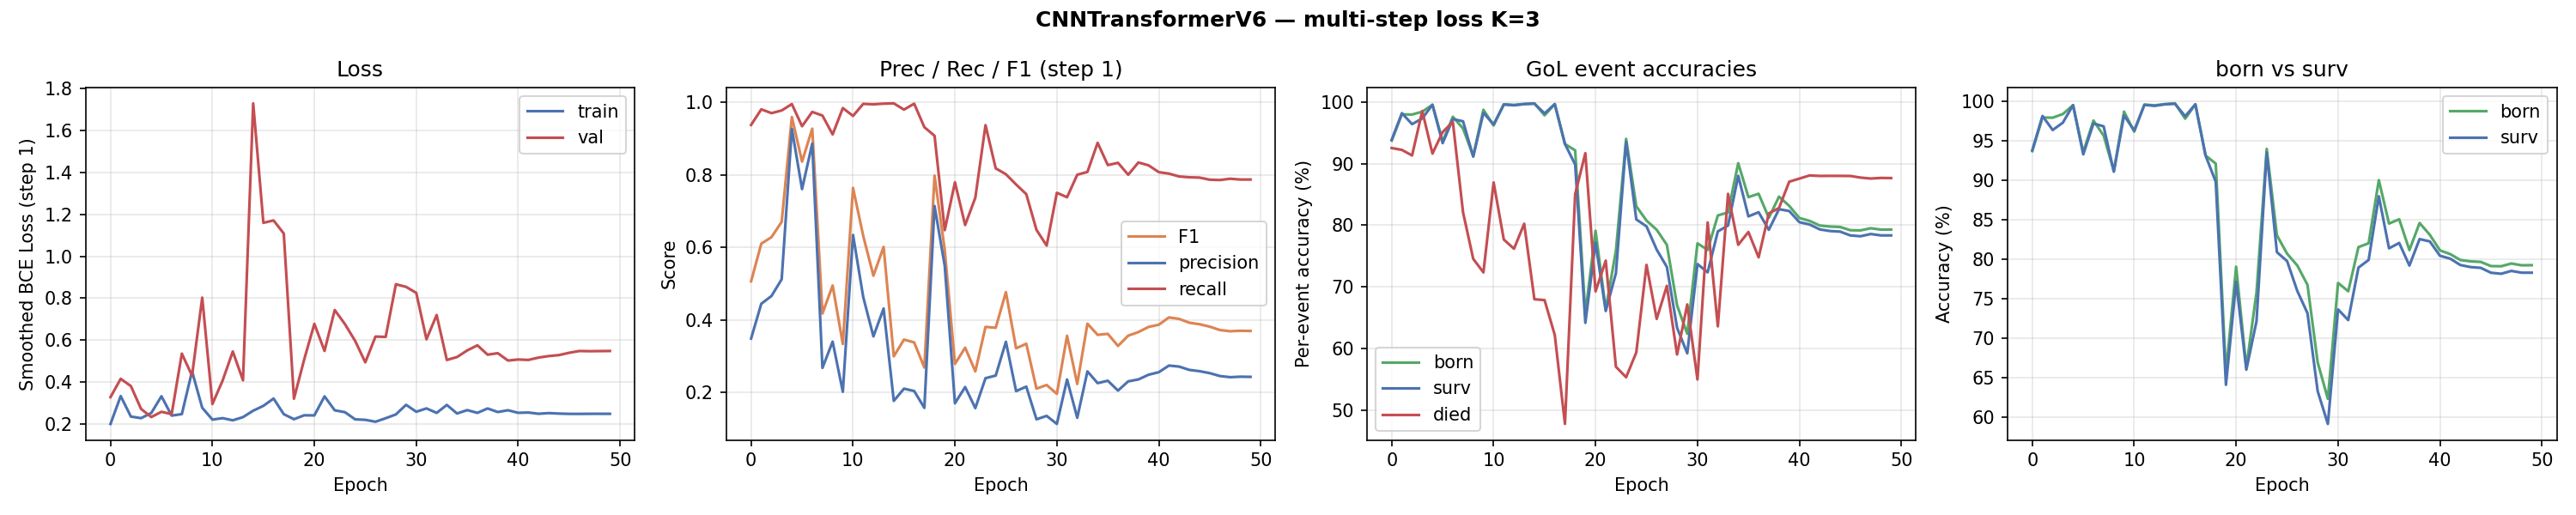
\includegraphics[width=0.85\textwidth]{figures/v6_loss.png}
  \caption{V6 training curves (STE multi-step, $K=3$). Precision collapses
  after an initial promising region around epoch 5 and never recovers.}
  \label{fig:v6-loss}
\end{figure}

A second attempt with STE at a lower learning rate ($1\mathrm{e}{-5}$) and
$K=2$ still diverged, with the same directional signature (precision
falling monotonically from epoch 1 to epoch 5), confirming the bias is
intrinsic to the STE gradient path rather than an optimization-stability
artifact.

\subsection{Working fix: scheduled sampling (V7)}

V7 replaces the STE hard/soft split with \emph{scheduled sampling}
\cite{bengio2015scheduled}: at each of the $K=3$ unrolled steps, the next
input is the model's own (hard, binarized) prediction with probability
$p$, or the ground-truth frame with probability $1-p$, where $p$ increases
linearly from $0$ to $1$ over training. Critically, gradients flow only
through the \emph{current} step's logits --- there is no gradient path
connecting step $t+1$'s loss back to step $t$'s prediction, which removes
the STE's compounding directional bias entirely.

V7 trains stably for all 50 epochs (Figure~\ref{fig:v7-loss}) and reaches
the best aggregate metrics of any single-step-warm-started model in this
study: validation loss $0.20114$, F1 $0.9985$, precision $99.7\%$, recall
$100\%$, and \emph{all three} per-event accuracies (born, survival, death)
at $99.7$--$100\%$. Qualitatively, the artifact of rollouts settling into
sparse grid-aligned dead patterns --- visible in V5/V6 rollouts on sparse
inputs --- disappears entirely.

\begin{figure}[htbp]
  \centering
  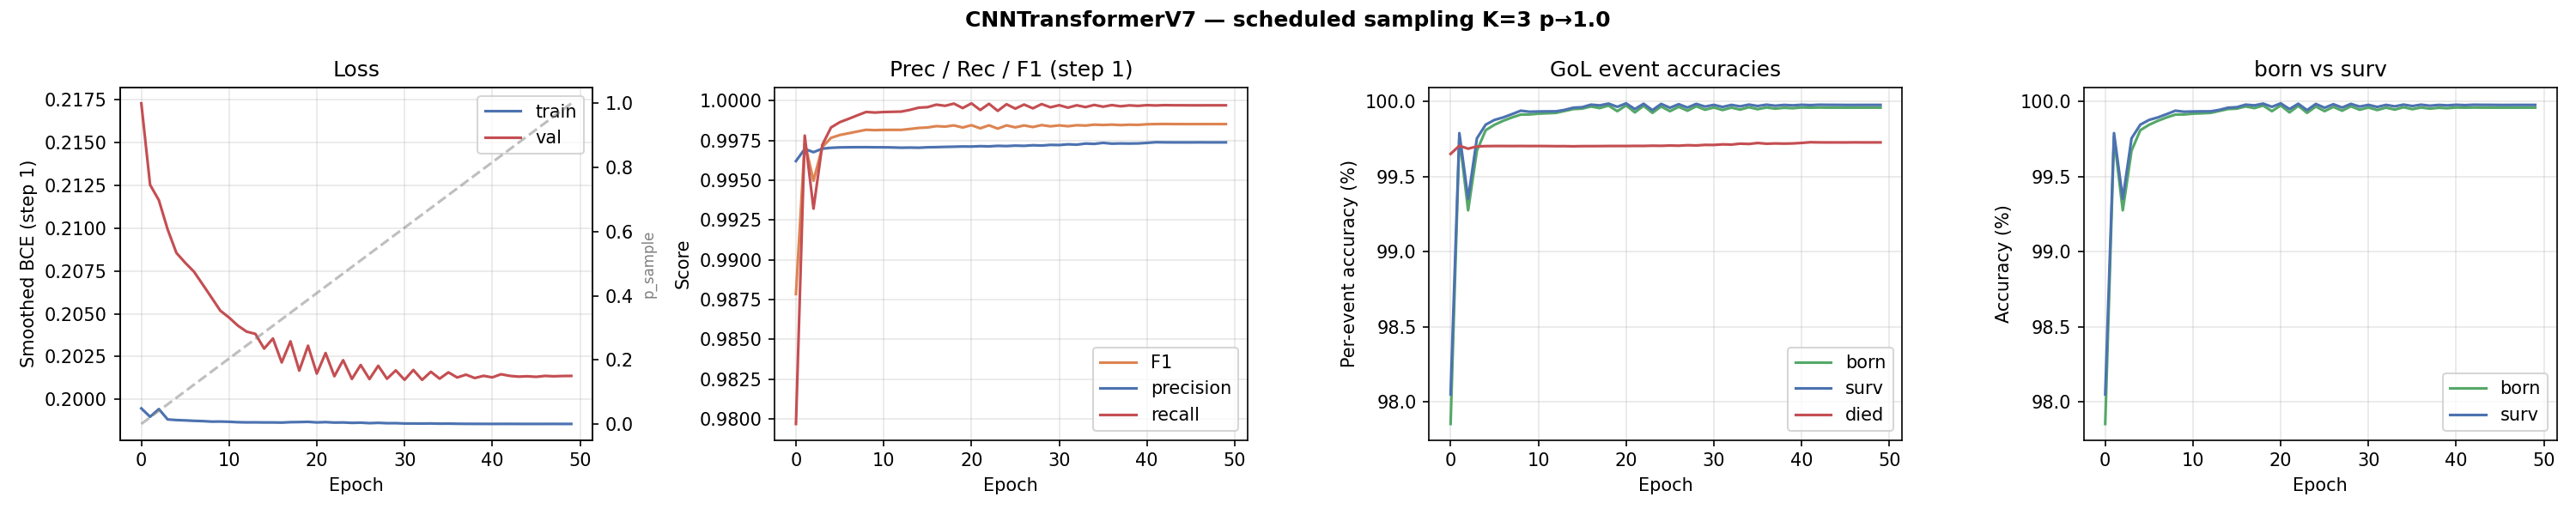
\includegraphics[width=0.85\textwidth]{figures/v7_loss.png}
  \caption{V7 training curves (scheduled sampling, $K=3$, $p: 0\to1$).
  Training is stable across all 50 epochs, with monotonically improving
  per-event accuracies.}
  \label{fig:v7-loss}
\end{figure}

\subsection{Targeted fine-tuning at high density (V8)}

Although V7's aggregate metrics are strong, a targeted failure search
(random grids across densities $0.02$--$0.80$, and 8 named small patterns,
seed-matched for reproducibility) finds that essentially all remaining
errors concentrate at high density ($d=0.80$), with roughly $100$ false
positives per grid on average.

V8 continues training V7's checkpoint for 30 further epochs with a dataset
that upsamples $d=0.65$ and $d=0.80$ trajectories by $3\times$ relative to
V7's dataset, while retaining the full range of lower densities (so the
model does not lose accuracy on sparse/medium configurations it already
handles well). This reduces the mean false-positive count at $d=0.80$ from
approximately $100$/grid to approximately $4.6$/grid --- a
$21\times$ improvement --- while aggregate metrics improve marginally
(validation loss $0.20064$, precision $100\%$, recall $99.9\%$).
Figure~\ref{fig:v7-v8-compare} shows a direct comparison of V7 and V8 on
one of the exact failure grids identified in the V7 failure search.

\begin{figure}[htbp]
  \centering
  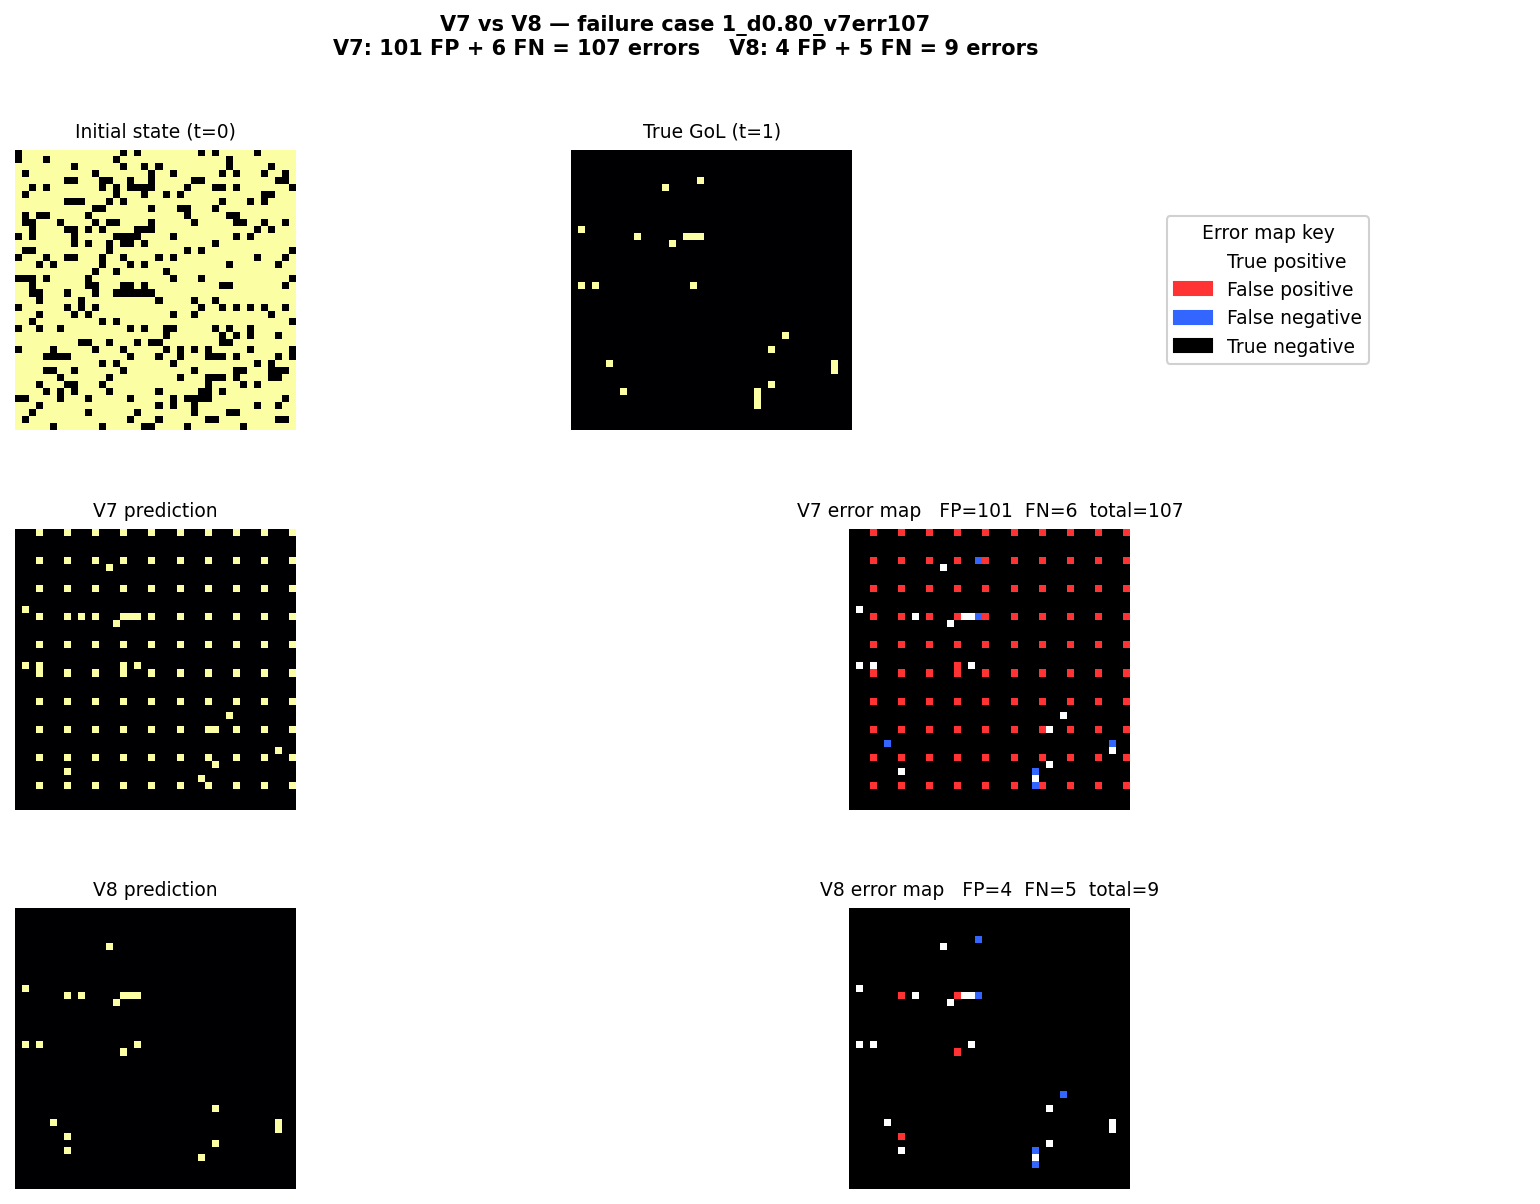
\includegraphics[width=0.95\textwidth]{figures/v7_v8_failure_compare.png}
  \caption{V7 vs.\ V8 on an identical $d=0.80$ failure grid found during the
  V7 failure search. V7 makes 107 errors (mostly false positives, visible as
  a diffuse grid-aligned speckle pattern); V8, fine-tuned with $3\times$
  more high-density data, makes substantially fewer errors on the same
  input.}
  \label{fig:v7-v8-compare}
\end{figure}

\subsection{Data scale-up regresses performance (V9)}

Given V8's improvement from more high-density data, we test whether scaling
\emph{all} data five-fold (approximately $546{,}200$ total training
examples, warm-started from V8) improves matters further. Aggregate
validation metrics remain similar to V8 (validation loss $0.20118$,
precision $99.7\%$, recall $99.6\%$), but per-grid error counts on the same
failure-search protocol \emph{worsen substantially}: false positives at
$d=0.80$ increase from V8's $2{,}296$ (across 500 grids) to $22{,}190$, and
false negatives at $d=0.50$ increase from $67$ to $6{,}948$.

This is the central negative result motivating Section~\ref{sec:results-table}:
\emph{aggregate validation metrics can look stable even as tail-case
behavior regresses sharply}, and simply scaling the training set does not
help once a model has saturated its representational capacity --- indeed it
can actively hurt, plausibly because the effective gradient signal from
over-represented high-density trajectories (each contributing many
alive-cell examples) skews optimization away from the sparse/medium regime
that was previously well-fit.

\begin{figure}[htbp]
  \centering
  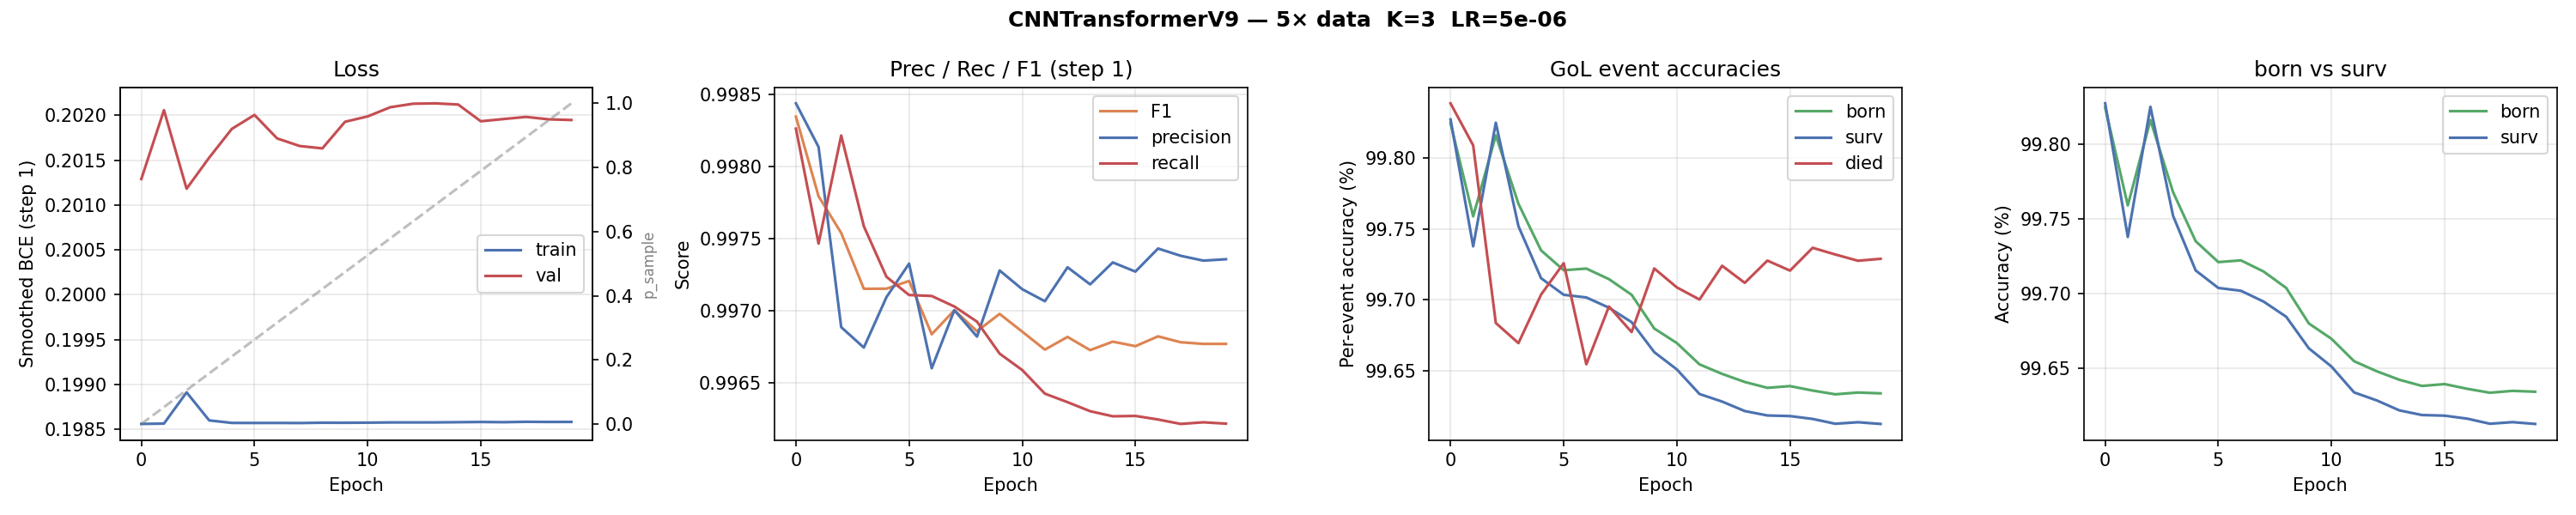
\includegraphics[width=0.85\textwidth]{figures/v9_loss.png}
  \caption{V9 training curves (5$\times$ data scale-up, warm-started from
  V8). Aggregate metrics look unremarkable, masking a substantial
  regression in per-grid tail-case error counts (see
  Table~\ref{tab:version-summary}).}
  \label{fig:v9-loss}
\end{figure}

\subsection{Scaling model capacity instead (V10)}

Rather than scaling data further, V10 scales the \emph{model}: doubling
$d_{\text{model}}$ ($64\to128$), doubling attention heads ($4\to8$), and
adding two Transformer layers ($4\to6$), for a total of $1{,}504{,}240$
parameters (5.15$\times$ V8's size). Because the embedding dimension
changes, V10 is trained \emph{from scratch} (V8/V9's weights cannot be
warm-started into a different-width model) using the same scheduled
sampling recipe and V8's dataset configuration (i.e., \emph{not} the 5$\times$
scaled-up V9 dataset).

V10 converges essentially immediately: by epoch 10 of 100, all metrics
(precision, recall, born, survival, death) reach $100.0\%$ and validation
loss reaches $0.19852$ --- notably \emph{below} the theoretical
label-smoothing floor achieved by any previous version, and the model
holds this exactly through epoch 100 (Figure~\ref{fig:v10-loss}).

\begin{figure}[htbp]
  \centering
  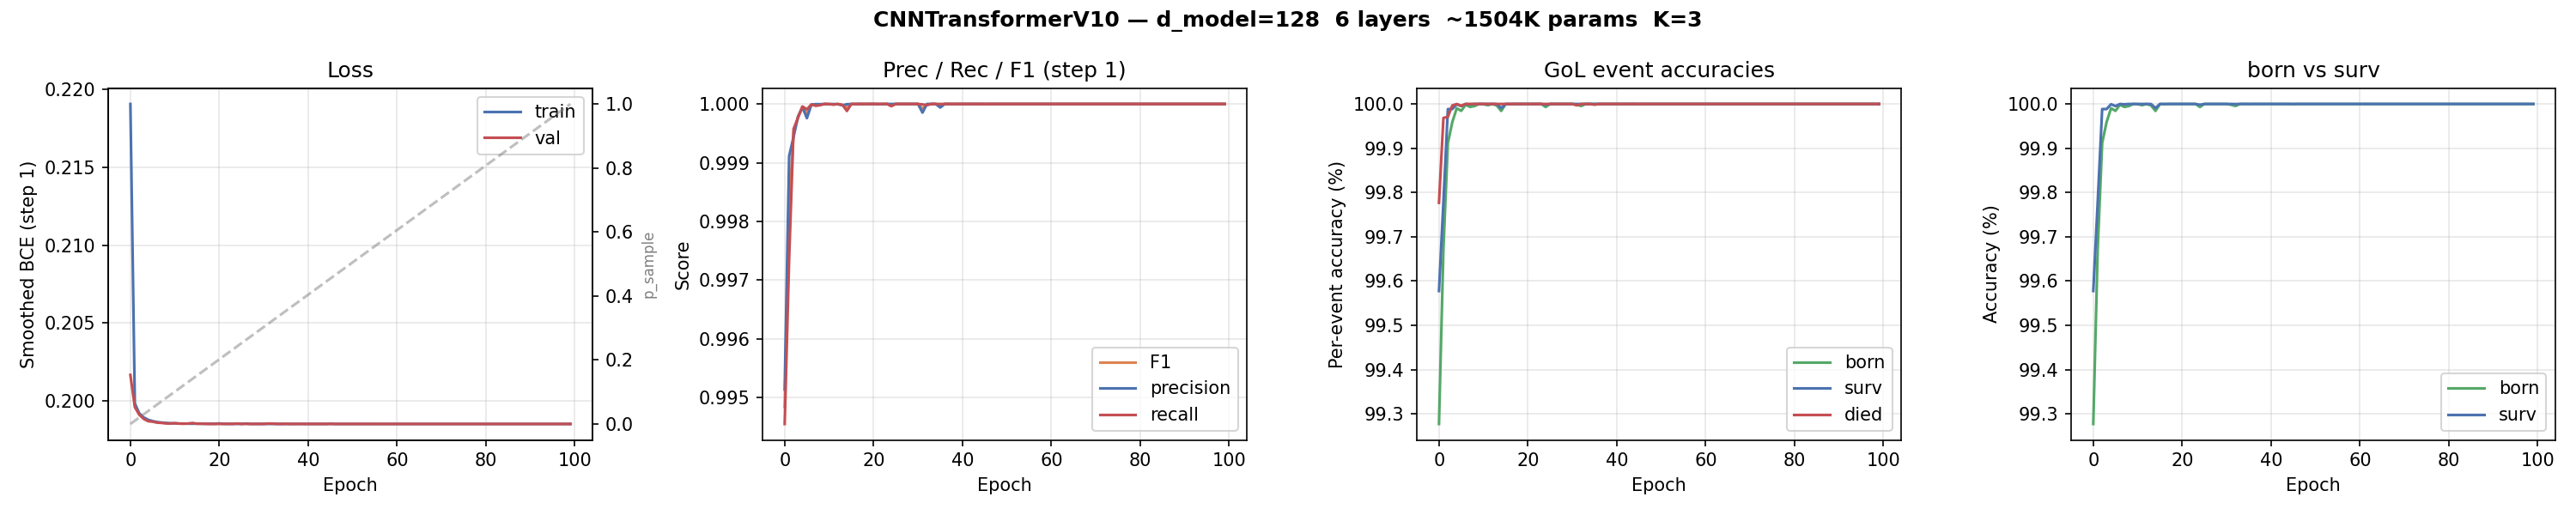
\includegraphics[width=0.85\textwidth]{figures/v10_loss.png}
  \caption{V10 training curves ($d_{\text{model}}=128$, 6 layers,
  $1.5$M params, trained from scratch). All metrics saturate at $100\%$
  by epoch 10 and remain stable through epoch 100.}
  \label{fig:v10-loss}
\end{figure}

Repeating the exact per-grid failure-search protocol used for V8/V9 (500
grids per density, densities $0.20$--$0.80$, fixed seed), V10 makes
\textbf{zero errors across all 2{,}500 evaluated grids} --- a qualitative
change from V8's thousands of residual errors at high density
(Table~\ref{tab:version-summary}, Figure~\ref{fig:v10-rollout}).

\begin{figure}[htbp]
  \centering
  \begin{subfigure}[t]{0.48\textwidth}
    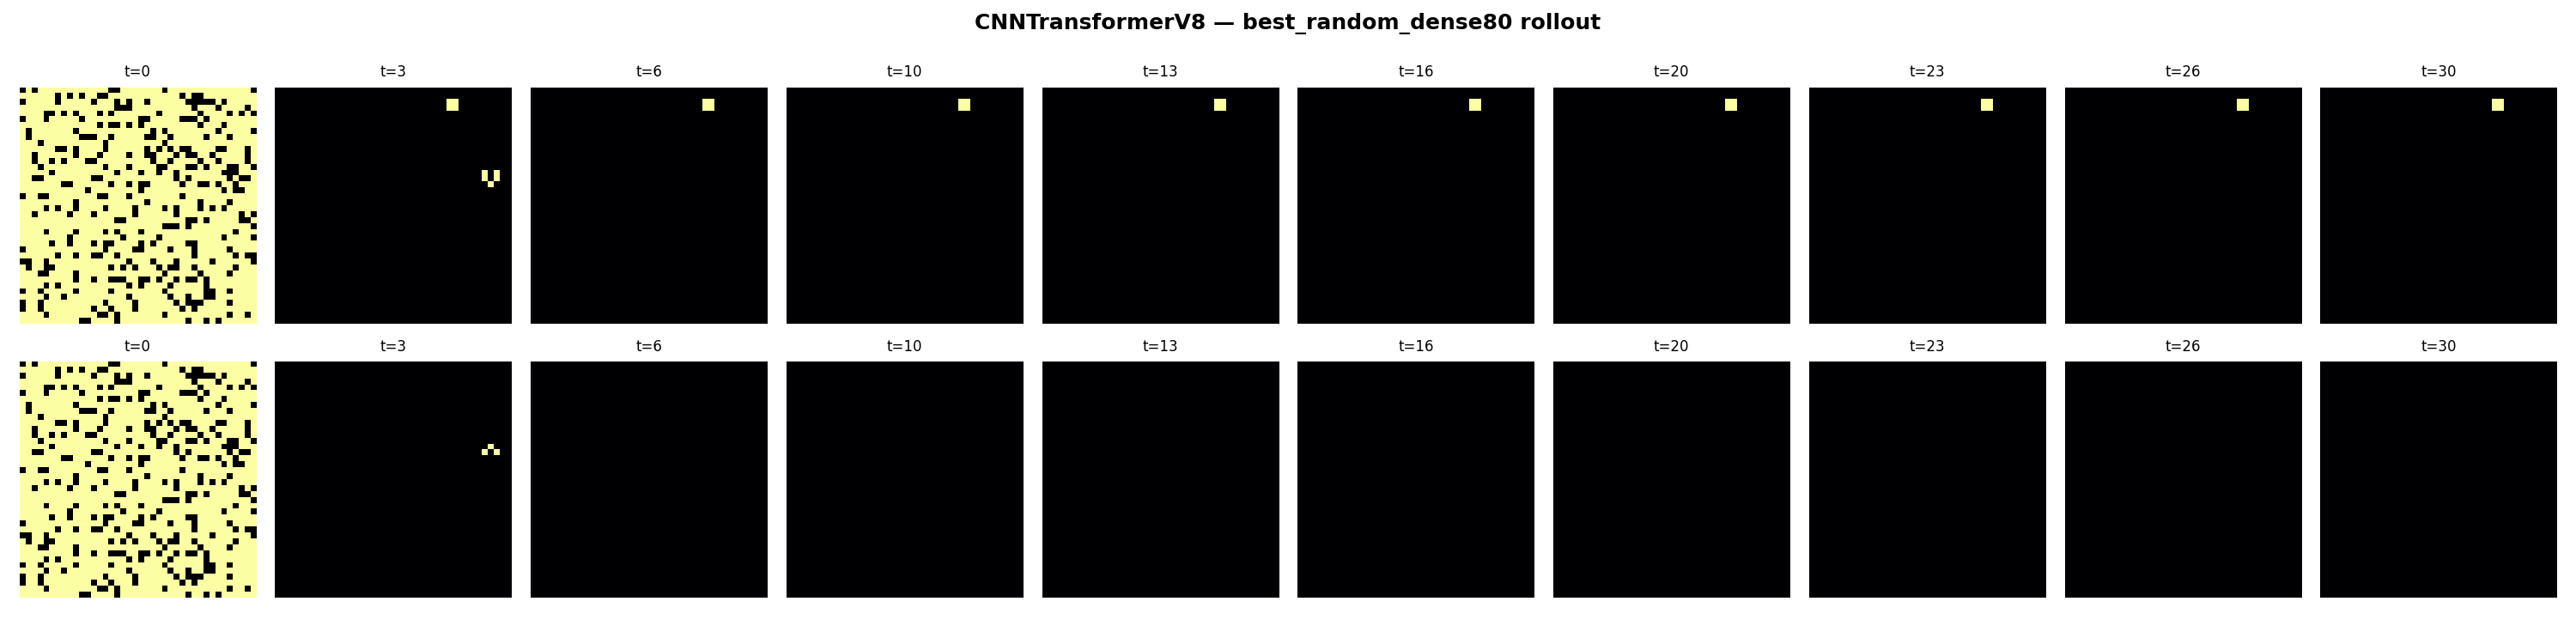
\includegraphics[width=\textwidth]{figures/v8_rollout_dense80.png}
    \caption{V8 (291K params)}
  \end{subfigure}
  \hfill
  \begin{subfigure}[t]{0.48\textwidth}
    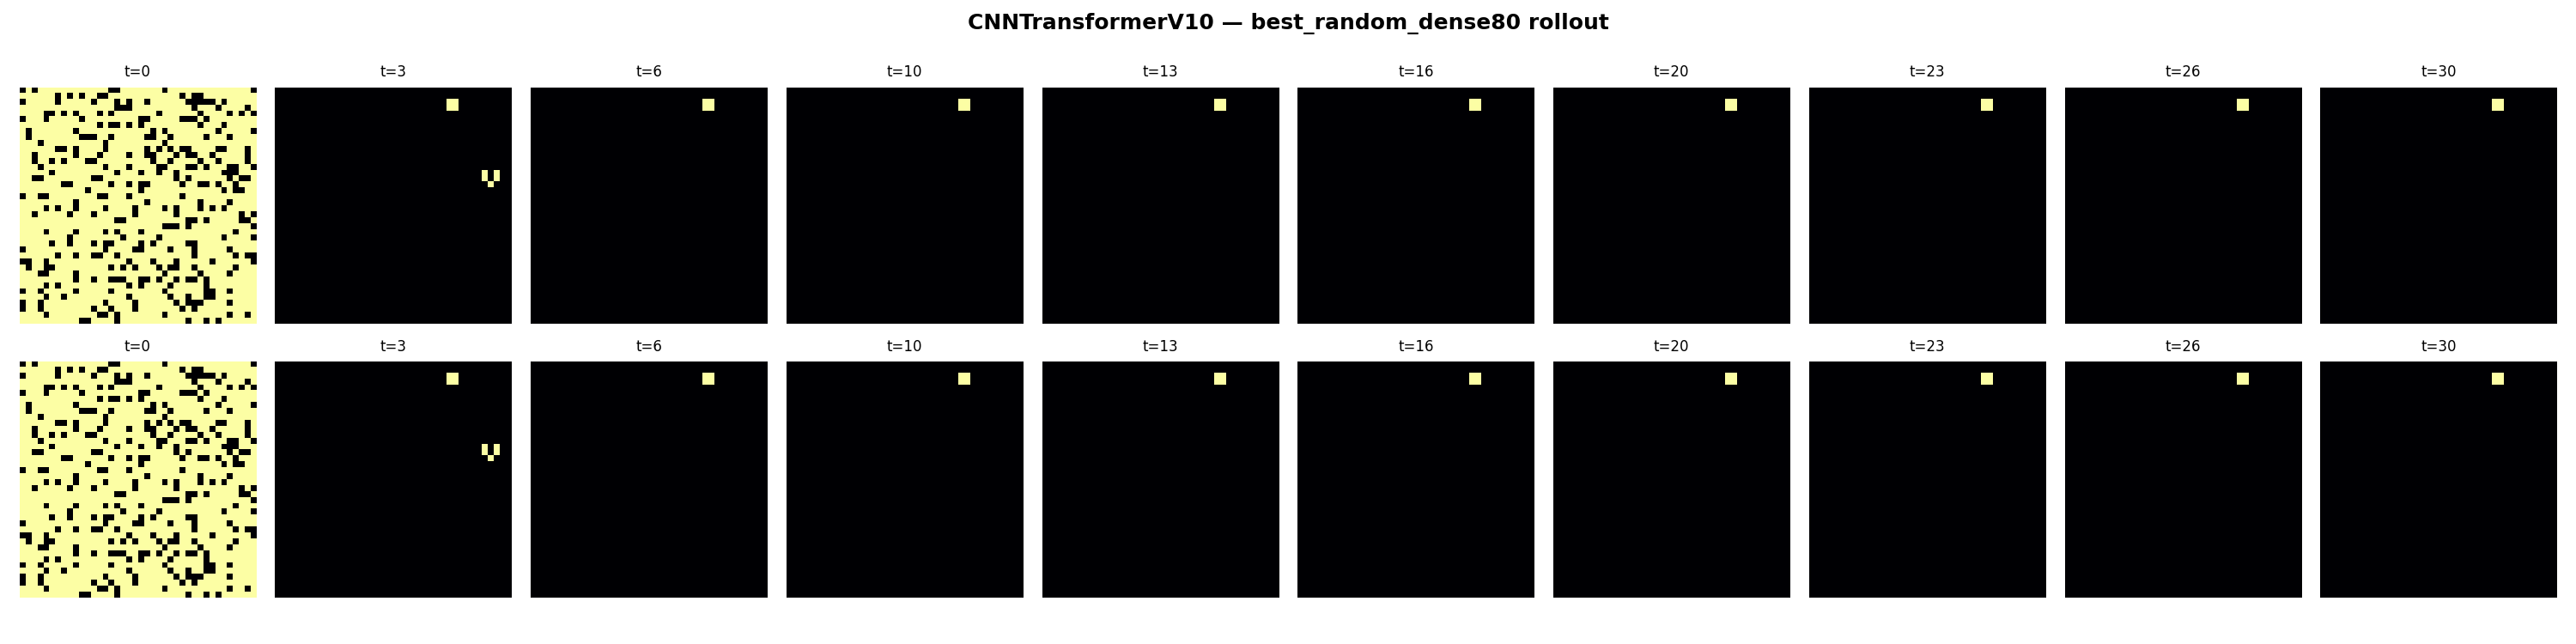
\includegraphics[width=\textwidth]{figures/v10_rollout_dense80.png}
    \caption{V10 (1.5M params)}
  \end{subfigure}
  \caption{30-step autoregressive rollout starting from a random $d=0.80$
  grid, true GoL trajectory (top row of each panel) vs.\ model prediction
  (bottom row).}
  \label{fig:v10-rollout}
\end{figure}

Taken together, V8 through V10 demonstrate that \emph{model capacity}, not
data volume, was the binding constraint at the $291$K-parameter scale: more
data of the same kind that a saturated model already sees plenty of does
not help (and can actively hurt), while more parameters directly resolve
the remaining tail-case errors.

\section{Summary of All Versions}
\label{sec:results-table}

Table~\ref{tab:version-summary} summarizes the full progression of models
discussed in Section~\ref{sec:training-evolution}. ``Per-grid errors''
figures (where available) come from a fixed failure-search protocol: 500
random grids at each of five densities ($0.20$, $0.35$, $0.50$, $0.65$,
$0.80$), same random seed across models, counting total false
positive + false negative cells summed over all 500 grids at each density.

\begin{table}[htbp]
\centering
\small
\resizebox{\textwidth}{!}{%
\begin{tabular}{lp{4.7cm}ccccl}
\toprule
Ver.\ & Key change & Best val loss & Prec.\ & Rec.\ & Born & Status \\
\midrule
V5 & Single-step teacher forcing (baseline) & 0.20125 & 99.4\% & 99.7\% & 93.8\% & Collapses under rollout \\
V6 & +STE multi-step ($K=3$) & 0.23421\textsuperscript{a} & 92.7\%\textsuperscript{a} & --- & 99.5\%\textsuperscript{a} & \textbf{Failed} --- diverges \\
V7 & STE $\to$ scheduled sampling & 0.20114 & 99.7\% & 100\% & 100\% & Stable, strong \\
V8 & +3$\times$ high-density upsample & 0.20064 & 100\% & 99.9\% & 99.9\% & Best per-grid accuracy (291K) \\
V9 & +5$\times$ all data & 0.20118 & 99.7\% & 99.6\% & 99.6\% & \textbf{Regressed} per-grid errors \\
V10 & 5.15$\times$ model size, from scratch & 0.19852 & 100\% & 100\% & 100\% & \textbf{Zero errors}, 2{,}500/2{,}500 grids \\
\bottomrule
\end{tabular}%
}
\caption{Version summary. \textsuperscript{a}V6's best epoch (5) before
divergence; the model never recovers after this point.}
\label{tab:version-summary}
\end{table}

\begin{table}[htbp]
\centering
\begin{tabular}{lrrrr}
\toprule
Density & V8 total errors & V9 total errors & V10 total errors \\
\midrule
0.20 & 0     & --   & 0 \\
0.35 & 192   & ---  & 0 \\
0.50 & 94    & 6{,}948\textsuperscript{b} & 0 \\
0.65 & 1{,}891 & ---  & 0 \\
0.80 & 3{,}358 & 22{,}190 & 0 \\
\bottomrule
\end{tabular}
\caption{Per-grid error counts (false positives + false negatives, summed
over 500 grids per density) for the three model sizes discussed in
Section~\ref{sec:training-evolution}. \textsuperscript{b}V9 figure is false
negatives specifically, quoted as reported during the original failure
comparison; full V9 error breakdown at other densities was not re-collected
after the regression was identified and model capacity scaling (V10) was
pursued instead.}
\label{tab:per-grid-errors}
\end{table}

The central empirical claim of this section is visible directly in
Table~\ref{tab:per-grid-errors}: V9's aggregate validation metrics
(Table~\ref{tab:version-summary}) are statistically indistinguishable from
V8's, yet its per-grid tail-case error count is an order of magnitude
\emph{worse}. This discrepancy would not have been visible from validation
loss or aggregate precision/recall alone --- it required a targeted,
density-stratified failure search to detect. We consider this the main
practical lesson of the V8--V10 progression: \emph{aggregate metrics on a
held-out validation set with the same distribution as training data can
silently hide severe regressions in specific, identifiable subpopulations
of the input space}, and per-subgroup error auditing is necessary to catch
this class of regression.

\section{Embedding Analysis}
\label{sec:embedding-analysis}

To understand what the learned patch representations encode, we extract two
embedding tensors per grid from the V8 and V10 models (Section~\ref{sec:architecture}):
the \textbf{pre-transformer} embedding (patch content projection $+$
learnable positional embedding, before attention) and the
\textbf{post-transformer} embedding (after the Transformer encoder mixes
information across all 100 patches). Both are $100 \times d_{\text{model}}$
tensors --- one $d_{\text{model}}$-dimensional vector per $4\times4$ patch,
arranged on a $10\times10$ grid.

\subsection{Static structure: patch norms and pairwise similarity}

For a fixed configuration, we visualize (i) the spatial map of
post-transformer embedding norms, $\|\text{emb}_i\|_2$ for each of the 100
patches, and (ii) the full $100\times100$ pairwise cosine similarity matrix
between all patches' embeddings.

\begin{figure}[htbp]
  \centering
  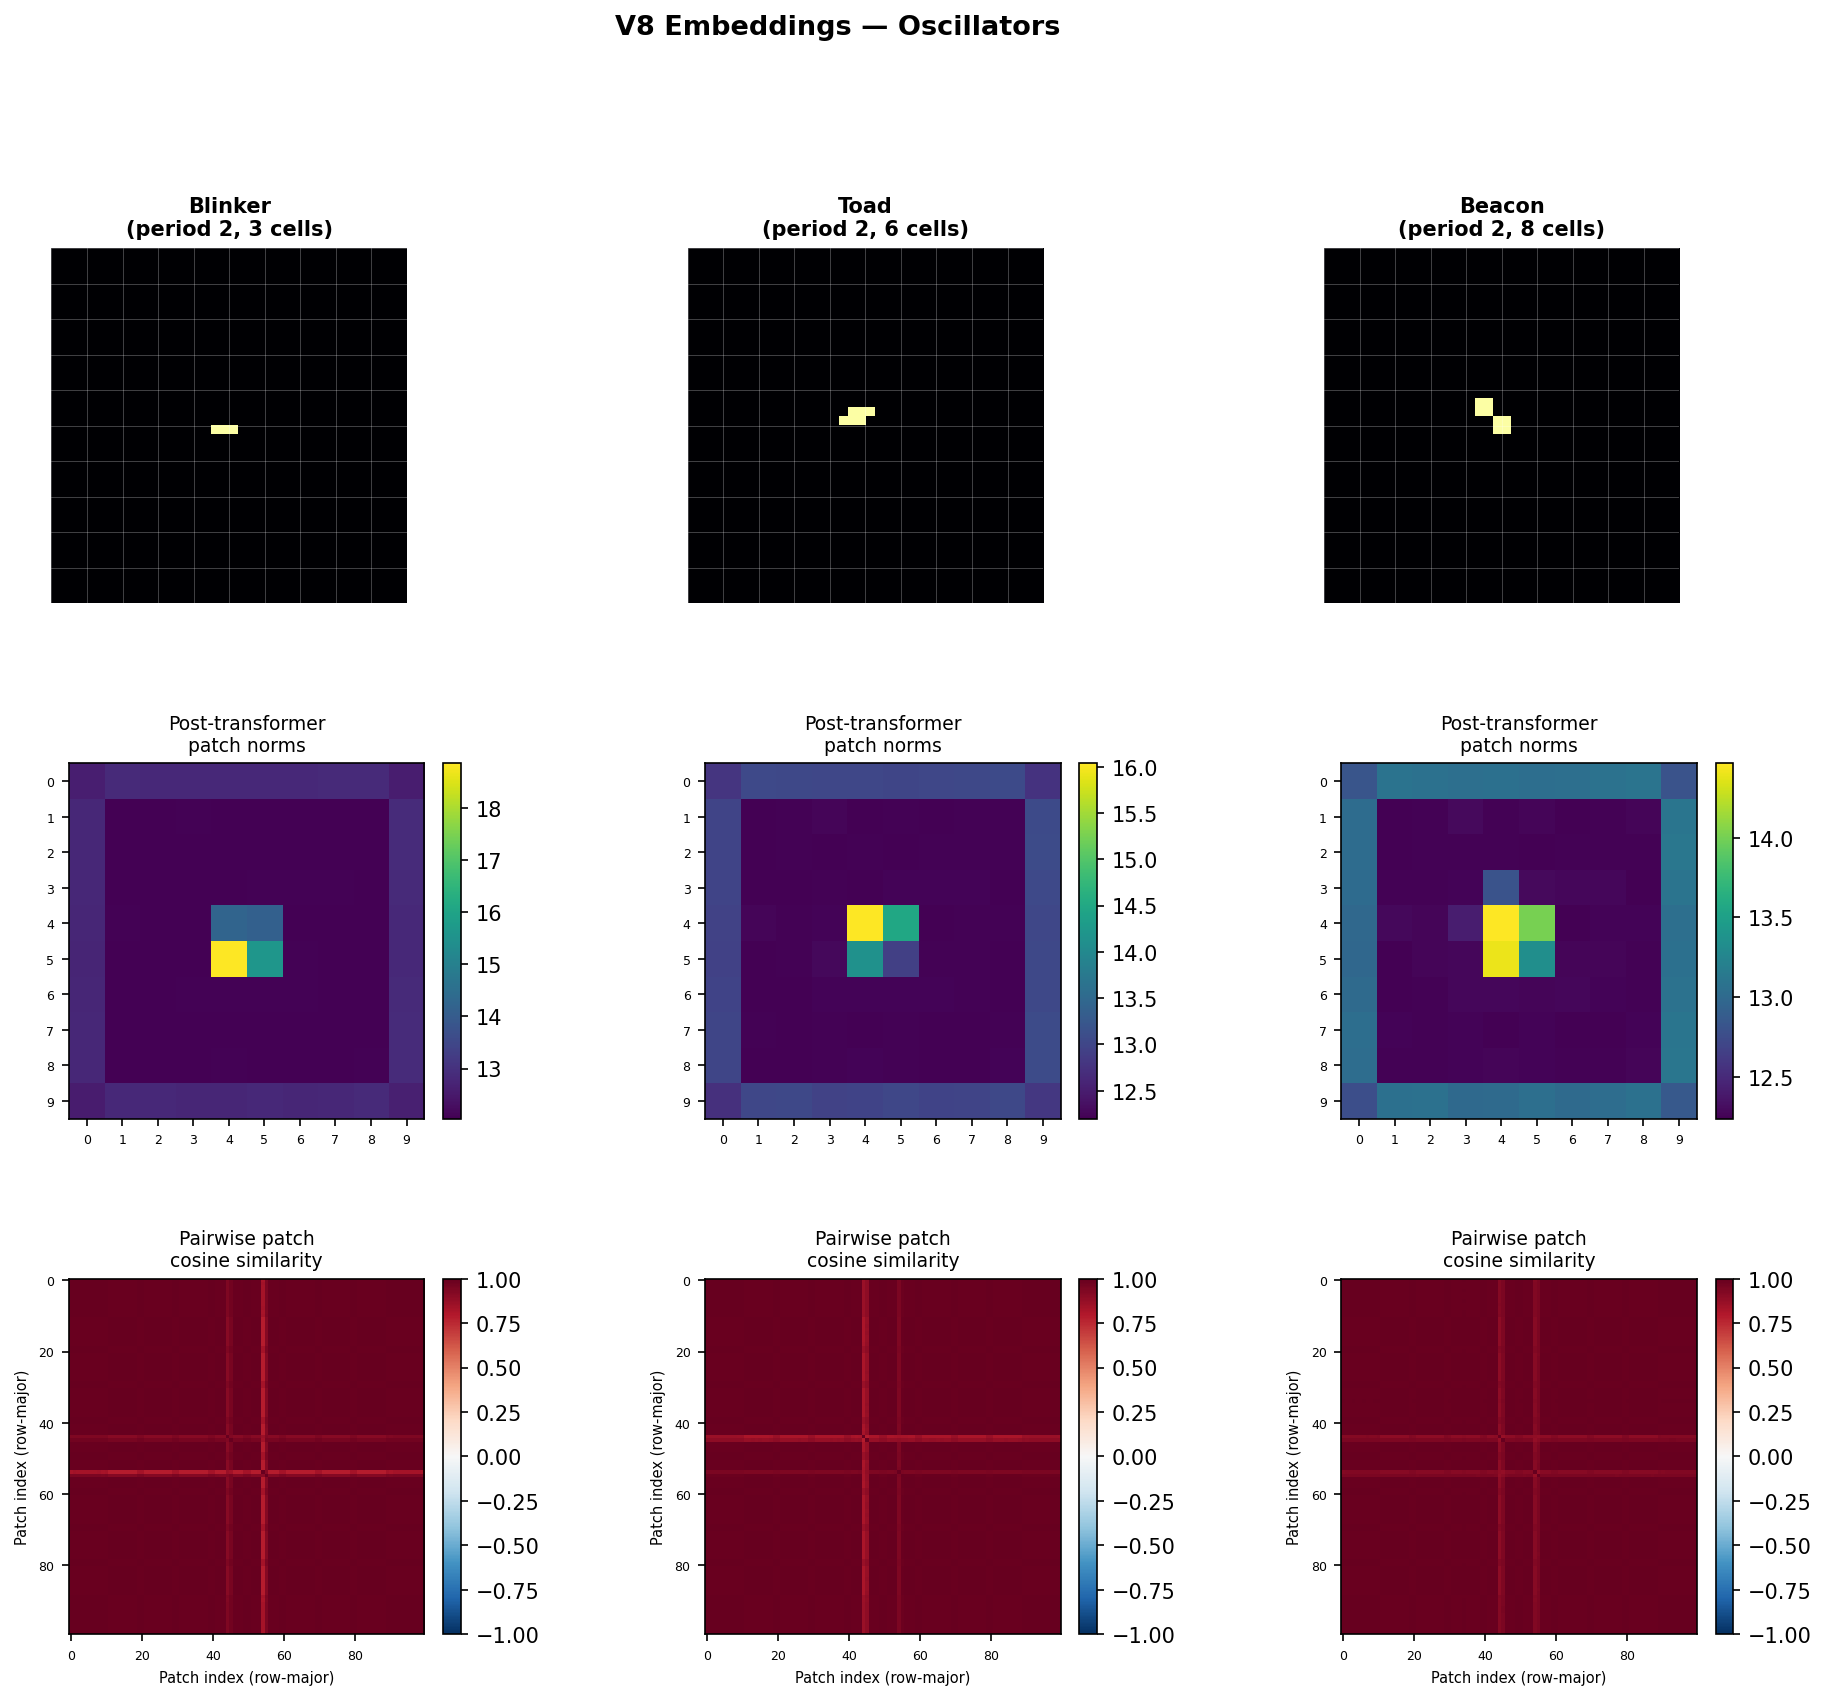
\includegraphics[width=\textwidth]{figures/gallery_v8_oscillators.png}
  \caption{V8 embeddings for three period-2 oscillators (blinker, toad,
  beacon). Top row: grid configuration. Middle row: post-transformer patch
  norm heatmap. Bottom row: $100\times100$ pairwise cosine similarity
  matrix. Sparse configurations produce a large, near-uniform block of
  mutually similar ``empty-patch'' embeddings, with only the 1--2 occupied
  patches standing apart.}
  \label{fig:gallery-oscillators}
\end{figure}

\begin{figure}[htbp]
  \centering
  \begin{subfigure}[t]{0.48\textwidth}
    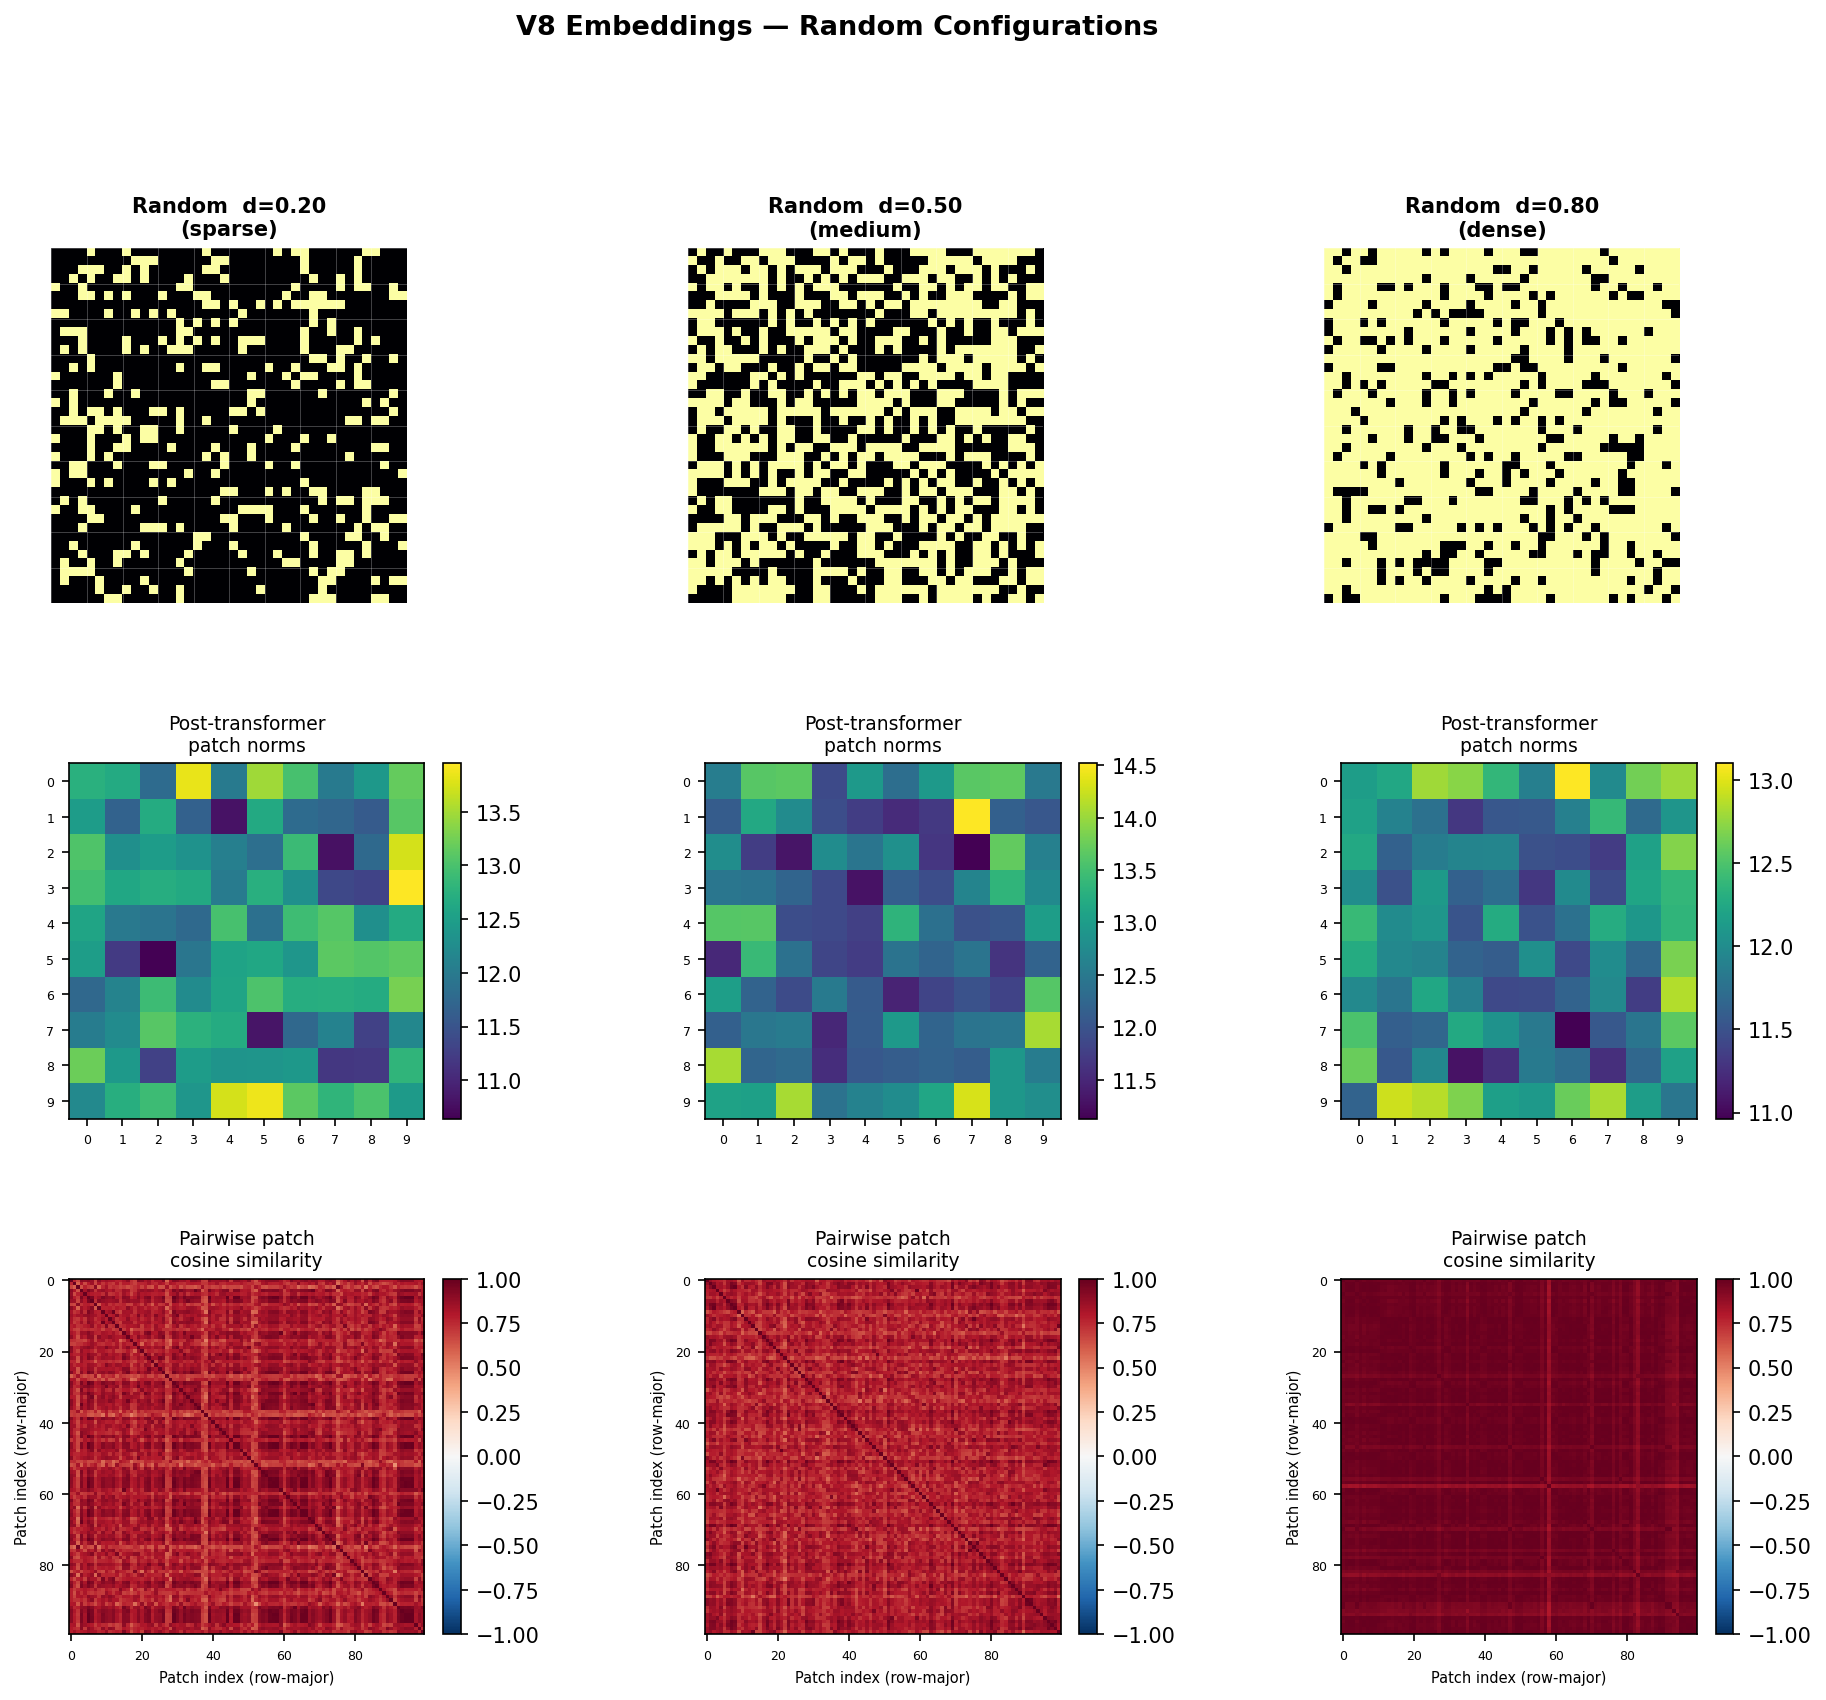
\includegraphics[width=\textwidth]{figures/gallery_v8_random.png}
    \caption{V8 (291K params)}
  \end{subfigure}
  \hfill
  \begin{subfigure}[t]{0.48\textwidth}
    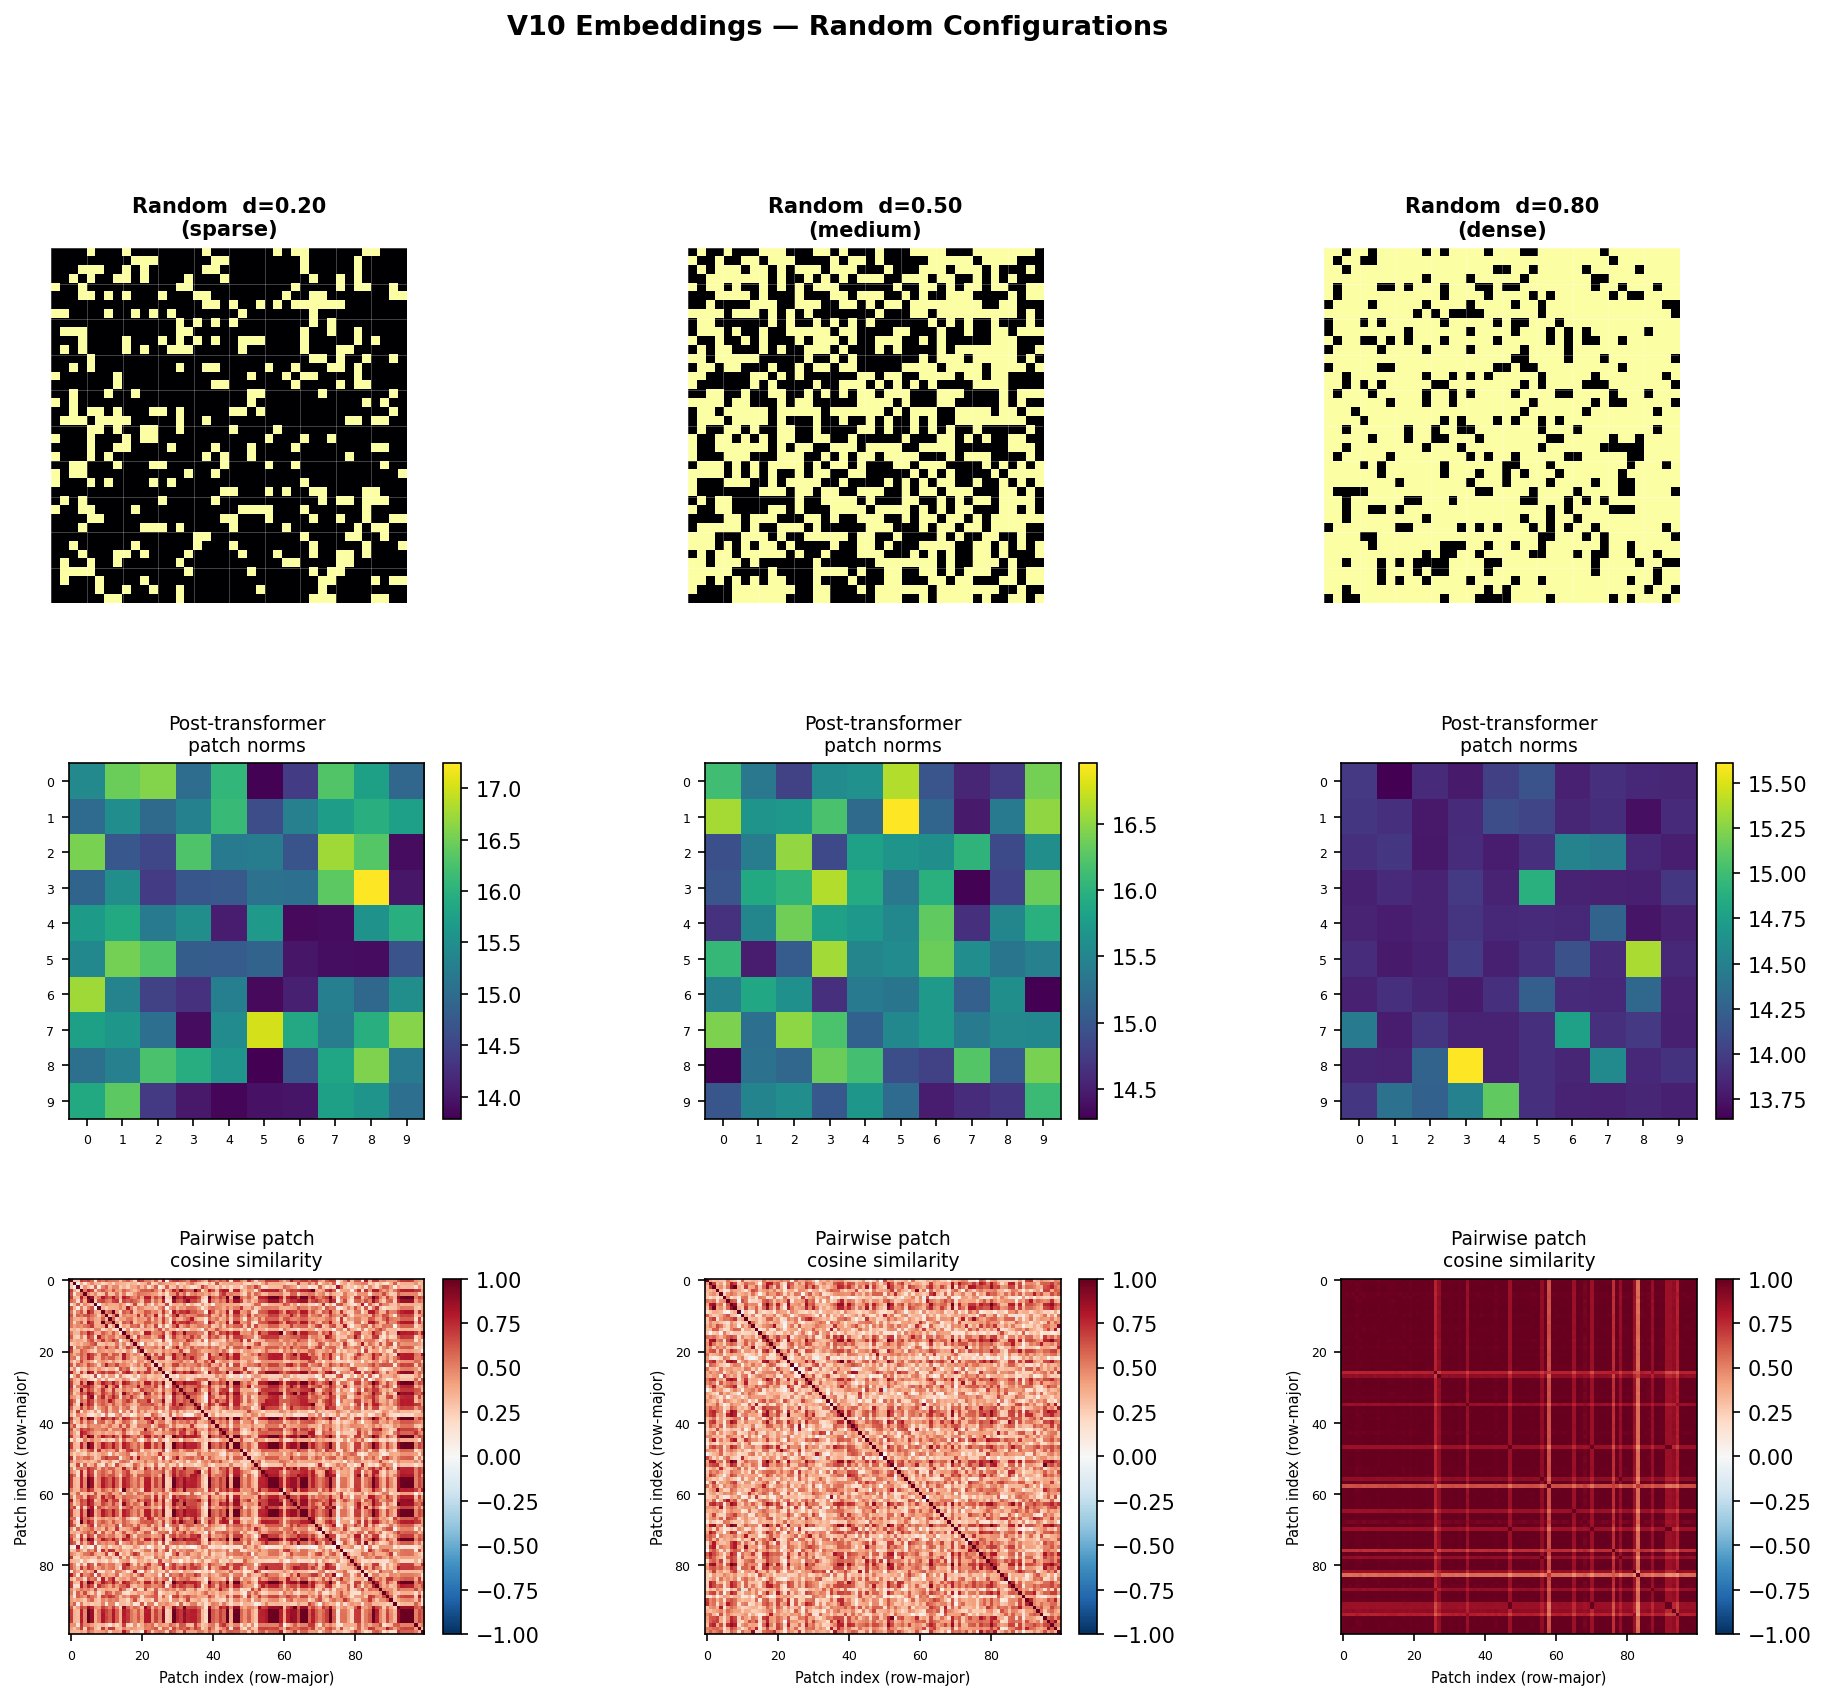
\includegraphics[width=\textwidth]{figures/gallery_v10_random.png}
    \caption{V10 (1.5M params)}
  \end{subfigure}
  \caption{Embeddings for random configurations at densities $0.20$, $0.50$,
  $0.80$ (left to right within each panel). As density increases, every
  patch carries genuine content, and the large ``empty-patch'' block seen
  in Figure~\ref{fig:gallery-oscillators} disappears, replaced by a more
  heterogeneous similarity structure.}
  \label{fig:gallery-random}
\end{figure}

Figure~\ref{fig:gallery-oscillators} shows that for sparse hand-placed
patterns, roughly 95--98 of the 100 patches are entirely empty and produce
near-identical embeddings (a large, uniformly high-similarity block in the
pairwise matrix), while the handful of occupied patches form a small,
distinct cluster. Figure~\ref{fig:gallery-random} shows this structure
eroding as density increases: at $d=0.80$, essentially every patch has
unique content, and the similarity matrix loses its block structure
entirely. This is a direct, visualizable signature of the sparse/dense
distinction that motivated the density-targeted fine-tuning in
Section~\ref{sec:training-evolution} (V8).

\subsection{Sensitivity to transformations}

We next measure how a patch's embedding changes under four families of
transformation applied to a fixed base configuration (glider, blinker, or
beacon): (i) $90^\circ/180^\circ/270^\circ$ rotation, (ii) horizontal/vertical
reflection, (iii) toroidal translation by 1 or 4 cells, and (iv) local
perturbation --- either flipping a single cell's state, or moving a single
live cell to an adjacent position. For each transformation we compute
$\Delta = \text{emb}(\text{transformed}) - \text{emb}(\text{original})$ per
patch, both pre- and post-transformer.

\begin{figure}[htbp]
  \centering
  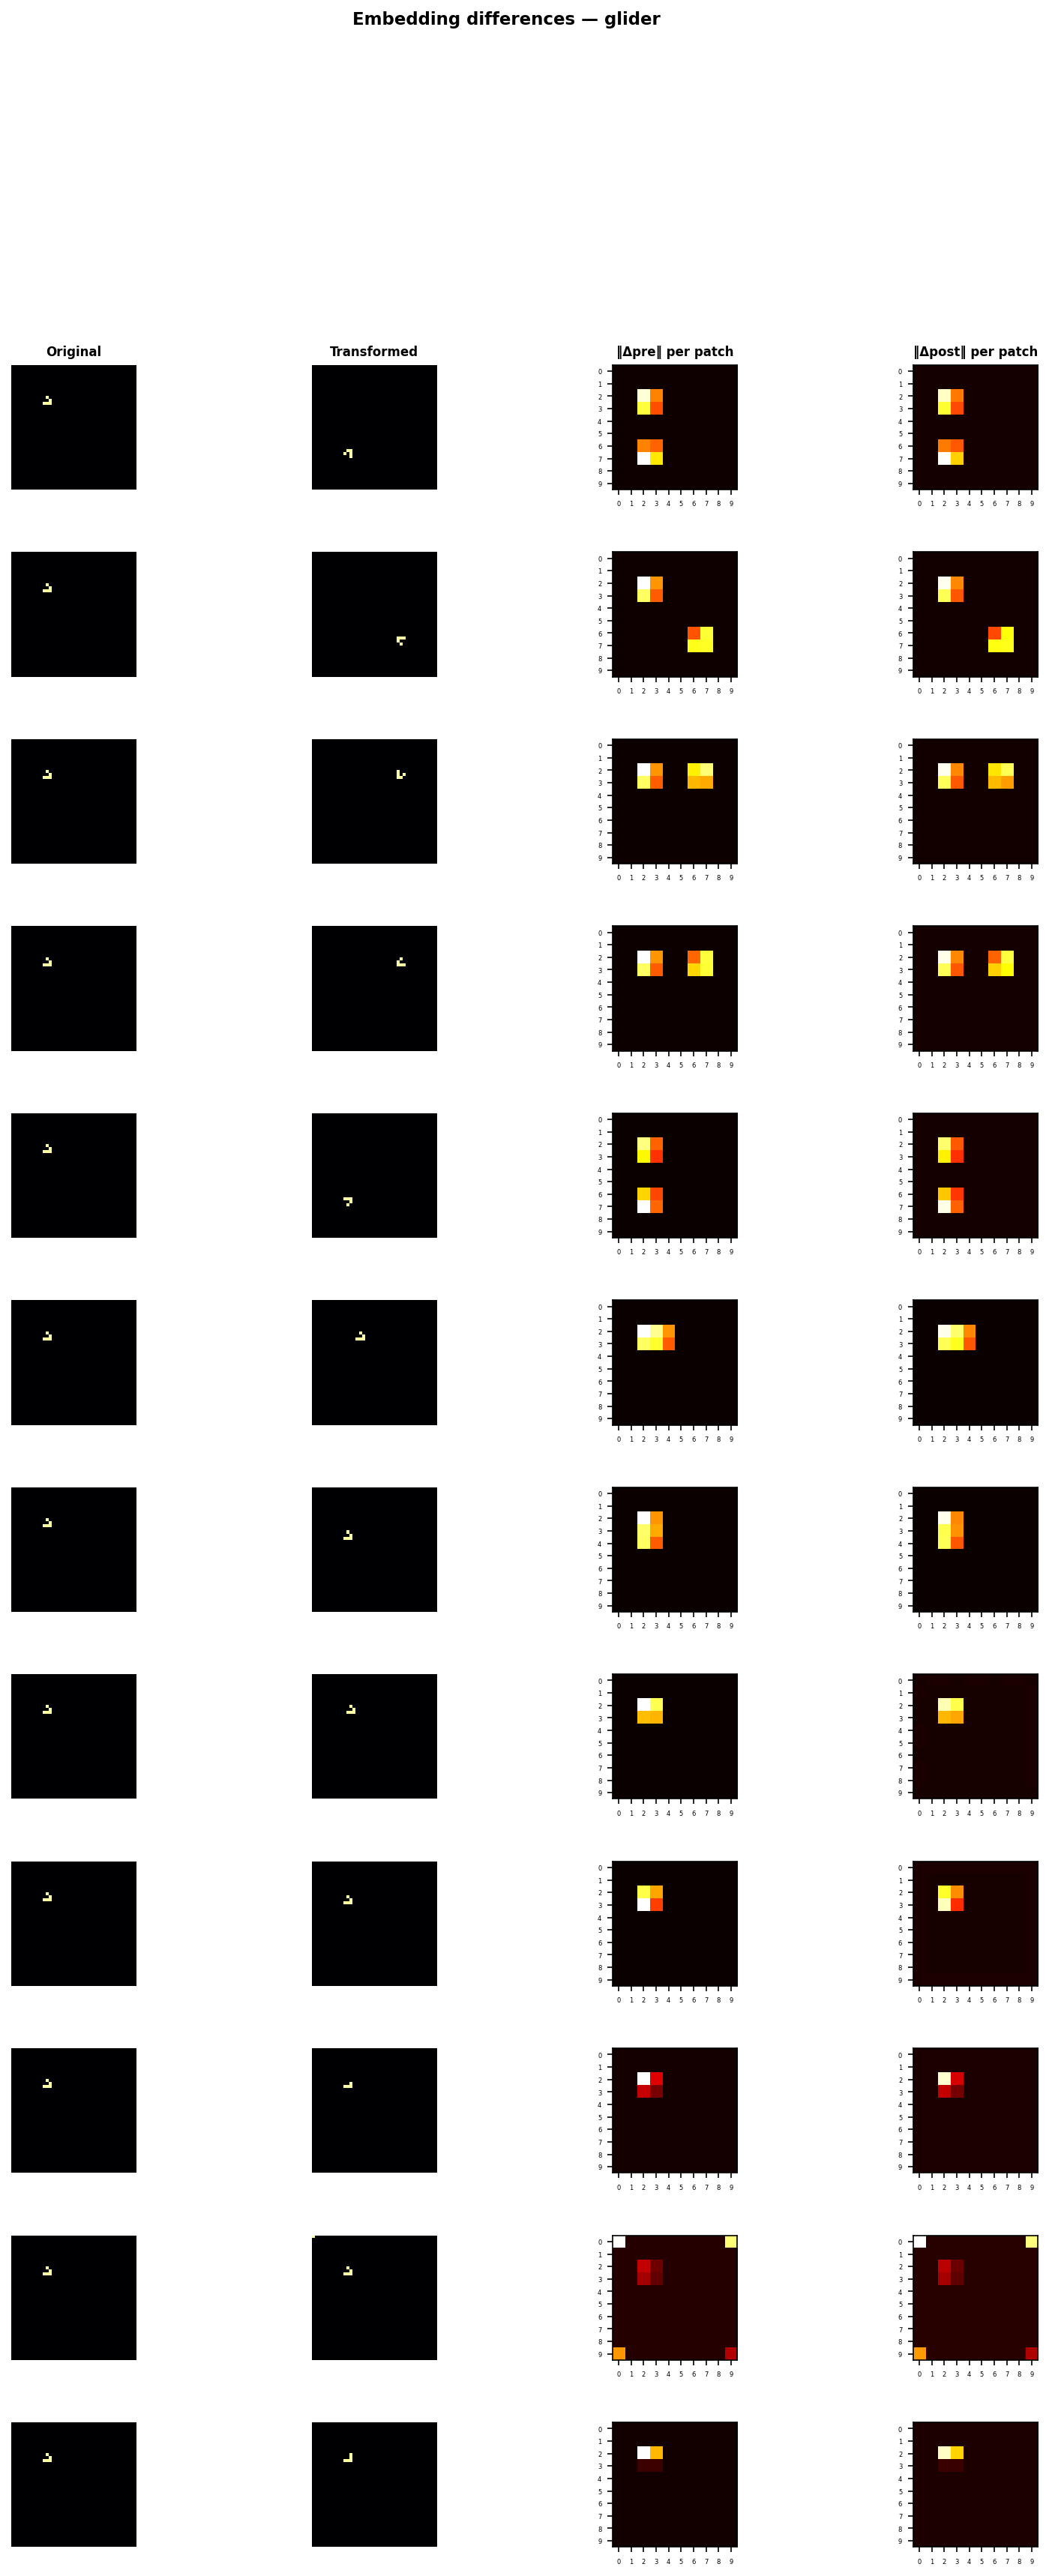
\includegraphics[height=0.75\textheight]{figures/embdiff_v8_deltanorms_glider.png}
  \caption{V8: per-patch embedding change $\|\Delta\|_2$ (pre- and
  post-transformer) for a glider under each transformation. Geometric
  transforms (rotation, reflection, coarse translation) perturb many
  patches at once because the pattern relocates to different absolute
  positions; single-cell perturbations affect only the one patch
  containing the perturbed cell.}
  \label{fig:embdiff-deltanorms}
\end{figure}

Table~\ref{tab:cosine-summary} (mean cosine similarity between original and
transformed post-transformer embeddings, averaged over all 100 patches)
quantifies the pattern visible in Figure~\ref{fig:embdiff-deltanorms}: sparse
patterns (glider) are nearly invariant to all transformations (cosine
similarity $\gtrsim 0.99$, since almost every patch is empty on both sides
of the transformation and empty patches encode almost identically
regardless of the grid's global content), while random grids show much
larger sensitivity to rotation, reflection, and coarse translation
($\approx 0.75$--$0.92$) because \emph{every} patch's absolute position
changes and the learnable positional embedding is position-specific, not
translation- or rotation-equivariant.

\begin{table}[htbp]
\centering
\begin{tabular}{lrrr}
\toprule
Transformation & Glider & Random ($d{=}0.35$) & Random ($d{=}0.65$) \\
\midrule
Rotate $90^\circ$        & 0.992 & 0.751 & 0.916 \\
Rotate $180^\circ$       & 0.991 & 0.744 & 0.909 \\
Flip horizontal          & 0.991 & 0.764 & 0.905 \\
Flip vertical            & 0.992 & 0.758 & 0.911 \\
Translate $+4$ cols      & 0.993 & 0.763 & 0.905 \\
Translate $+1$ col       & 0.996 & 0.780 & 0.924 \\
Cell flip (alive$\to$dead) & 0.9996 & --- & --- \\
Cell flip (dead$\to$alive) & 0.9988 & --- & --- \\
Cell move (1 step)         & 0.9987 & --- & --- \\
\bottomrule
\end{tabular}
\caption{Mean post-transformer cosine similarity between original and
transformed embeddings, V8. Sparse configurations are nearly invariant to
all transformations; dense random grids are substantially more sensitive to
geometric transforms, because the learnable absolute positional embedding
breaks exact translation/rotation equivariance.}
\label{tab:cosine-summary}
\end{table}

\subsection{Cross-transformation structure and geometry}

To ask whether different transformations perturb the embedding space in
\emph{similar directions}, we flatten each transformation's full
$\Delta \in \mathbb{R}^{100 \times d_{\text{model}}}$ vector and compute
pairwise cosine similarity across all transformations
(Figure~\ref{fig:embdiff-crosssim}). We additionally project the 100 patch
embeddings (original and every transformed version) into the top-2
principal components of the original configuration's embedding set
(Figure~\ref{fig:embdiff-pca}), to visualize how occupied patches move
through representation space under each transformation while the empty-patch
cluster remains essentially fixed.

\begin{figure}[htbp]
  \centering
  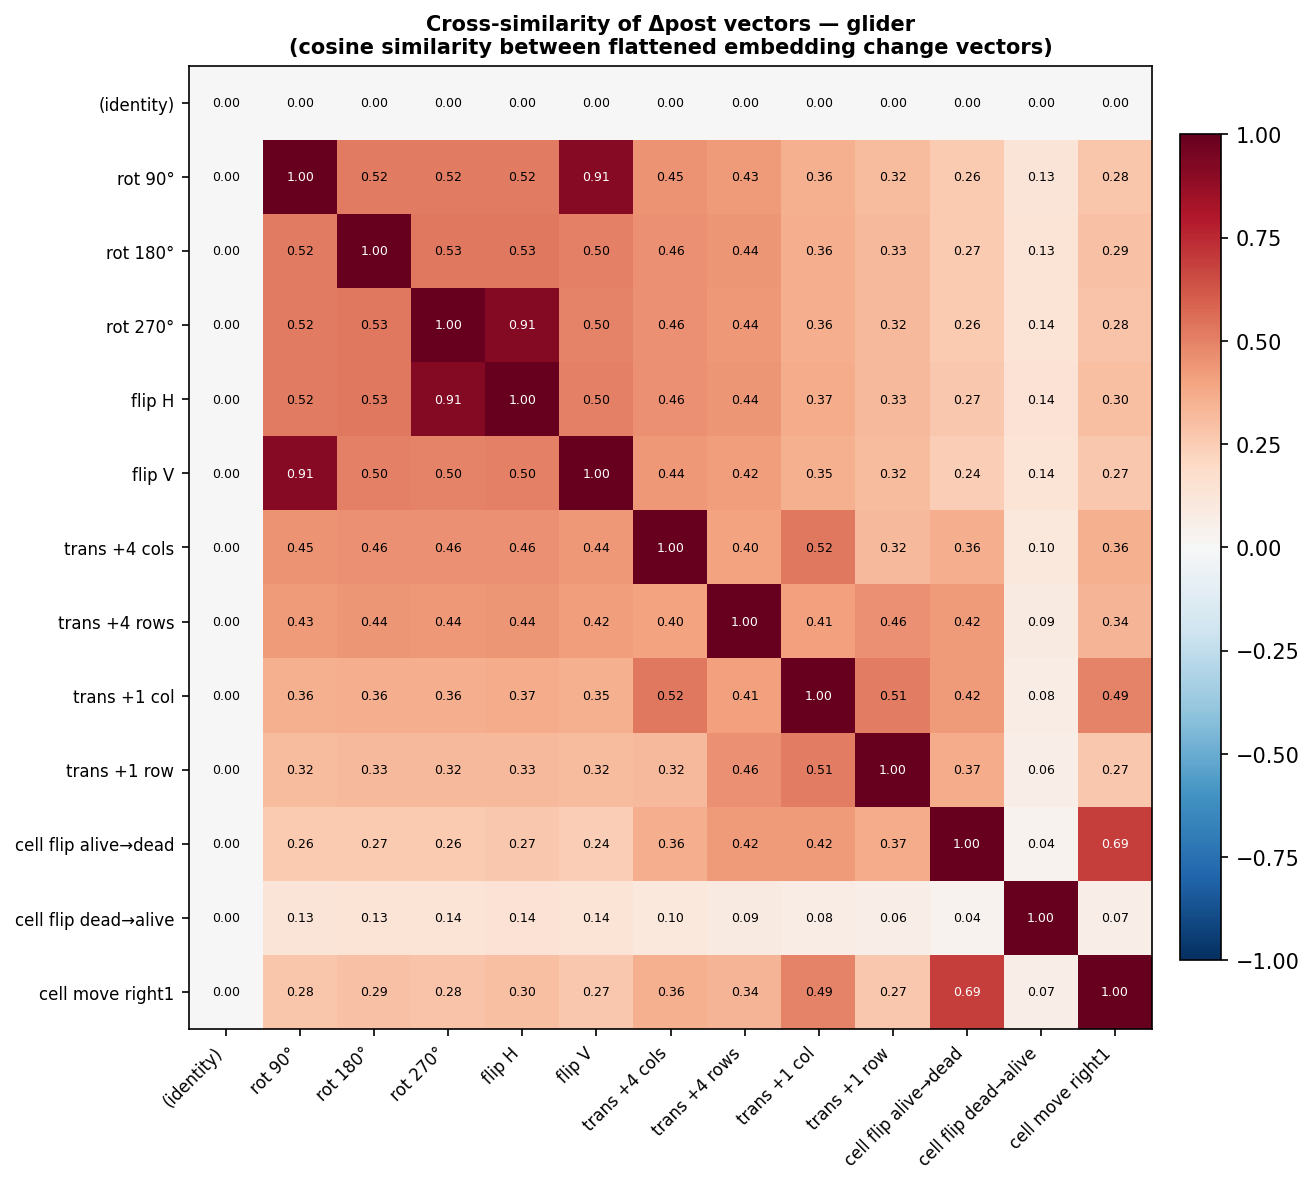
\includegraphics[width=0.7\textwidth]{figures/embdiff_v8_crosssim_glider.png}
  \caption{V8: cosine similarity between the flattened $\Delta_{\text{post}}$
  vectors of every pair of transformations (glider base pattern). Values
  near $1$ indicate two transformations perturb the embedding space in
  nearly the same direction; values near $0$ indicate unrelated
  perturbation directions.}
  \label{fig:embdiff-crosssim}
\end{figure}

\begin{figure}[htbp]
  \centering
  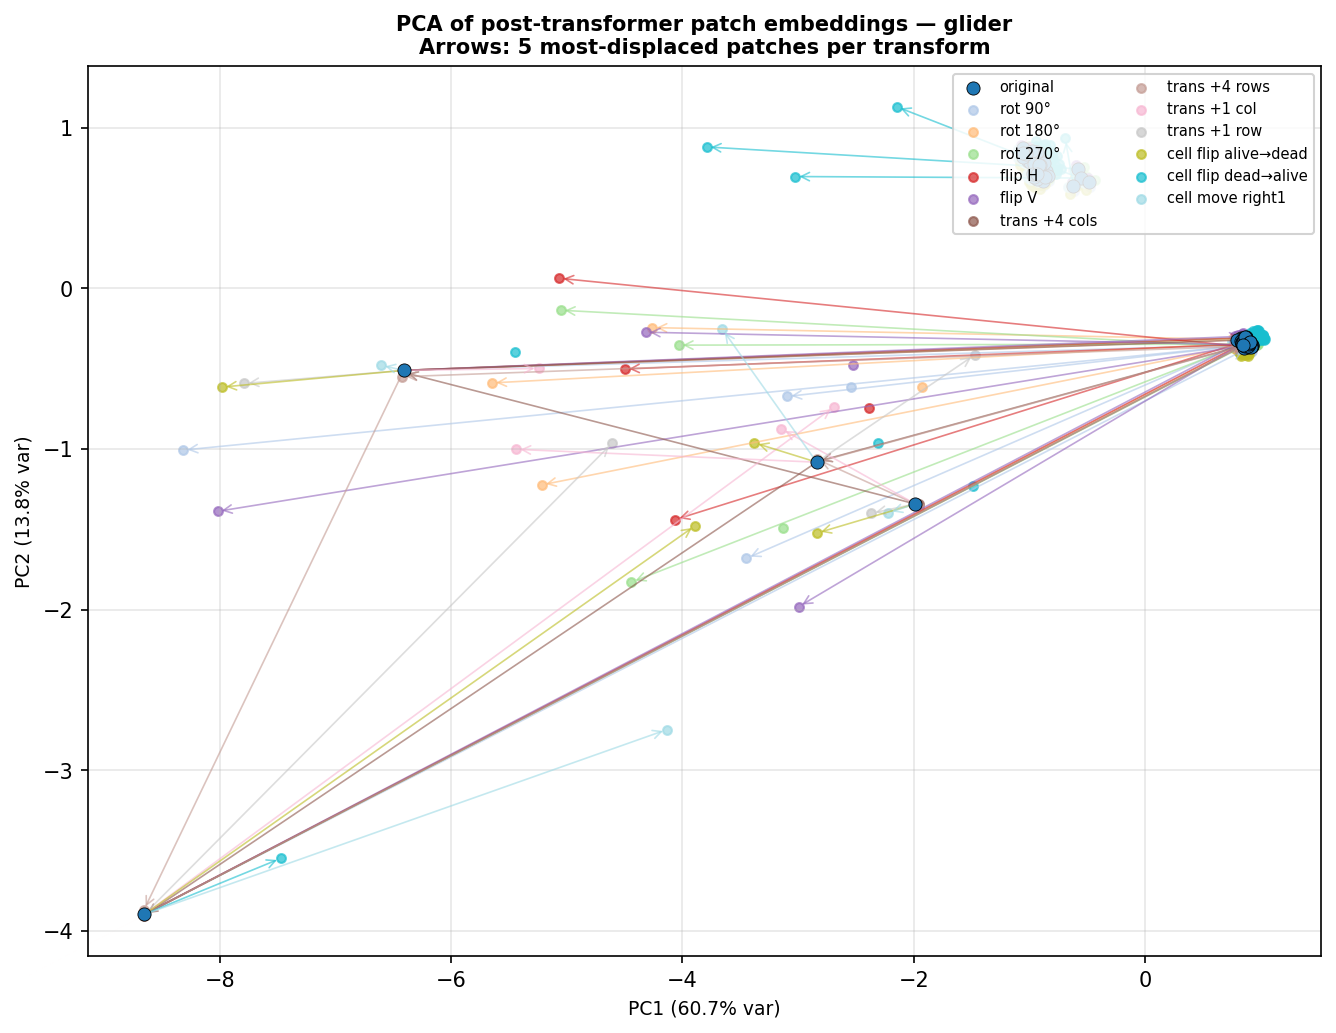
\includegraphics[width=0.7\textwidth]{figures/embdiff_v8_pca_glider.png}
  \caption{V8: PCA projection (fit on the original glider's 100 patch
  embeddings) of the embeddings under every transformation. The large
  central cluster is the $\sim$95 empty patches, essentially stationary
  across all transformations; arrows trace the 5 most-displaced patches per
  transformation, showing where the occupied-patch information moves to
  under each transform.}
  \label{fig:embdiff-pca}
\end{figure}

Qualitatively, geometric transformations (rotation, reflection) that share
the dihedral symmetry group used in data augmentation
(Section~\ref{sec:architecture}) tend to produce more mutually correlated
$\Delta$ vectors than translation does, consistent with the model having
been explicitly trained to be robust to (though not embedding-invariant
under) $D_4$ transformations, while translation invariance was never
encouraged during training.

\section{Activation-Function Inductive Bias}
\label{sec:verification}

\subsection{Motivation: Polynomial Kolmogorov-Arnold Networks}

Ahmed \& Davis \cite{ahmed2026polynomial} study why small neural networks
struggle to \emph{learn} the GoL transition rule despite minimal networks
being known to \emph{represent} it exactly with only a handful of
hand-set parameters \cite{springer2021minimal}. They argue that the GoL
update is a non-monotonic function of live-neighbor count $N$ --- flat at
zero for $N \in \{0,1\}$, rising sharply for $N \in \{2,3\}$, and flat at
zero again for $N \geq 4$ --- which a monotonic activation such as ReLU can
only approximate piecewise, requiring many units and a fortunate
initialization (a ``winning ticket'') to succeed reliably. They show that
replacing ReLU with a \emph{learnable second-degree polynomial} activation,
\[
  \phi(x) = w_0 + w_1 x + w_2 x^2,
\]
lets a minimal CNN --- one $3\times3$ circularly-padded convolution, one
$1\times1$ convolution, and a final $1\times1$ convolution with sigmoid
output --- learn GoL reliably on a $32\times32$ toroidal grid, whereas the
same architecture with ReLU activation fails almost completely.

\subsection{Independent reproduction}
\label{sec:reproduction}

Before attempting to transfer this idea into our larger CNN-Transformer, we
independently verify the paper's central claim on our own $40\times40$
toroidal setup, using a from-scratch reimplementation (available in
\texttt{poly\_activation\_verify/}, kept deliberately separate from the main
codebase) with no dependency on our own GoL simulator or model code. We
build the minimal $L(1,m{=}1)$ architecture described above and train two
variants --- identical in every respect except the activation function used
at the two hidden activation sites --- with plain single-step teacher
forcing (binary cross-entropy, Adam, learning rate $10^{-3}$, batch size
$8$) on a small dataset of 100 training / 20 validation random grids
(density sampled uniformly in $[0.1, 0.9]$), across 10 random seeds per
activation.

\begin{table}[htbp]
\centering
\begin{tabular}{lrrrr}
\toprule
Activation & Parameters & Success rate & Mean epochs to converge & Mean final accuracy \\
\midrule
ReLU       & 25 & 1/10  & 159.0 (of successful run) & 89.39\% \\
Polynomial & 34 & 10/10 & 185.6 & 100.00\% \\
\bottomrule
\end{tabular}
\caption{Reproduction of Ahmed \& Davis \cite{ahmed2026polynomial} on our
own $40\times40$ toroidal grid and independent implementation. Parameter
counts (25 and 34) match the paper's reported minimal-network sizes
exactly. ``Success'' is defined as reaching $\geq 99.99\%$ validation cell
accuracy for two consecutive epochs, within 500 epochs.}
\label{tab:relu-vs-poly}
\end{table}

\begin{figure}[htbp]
  \centering
  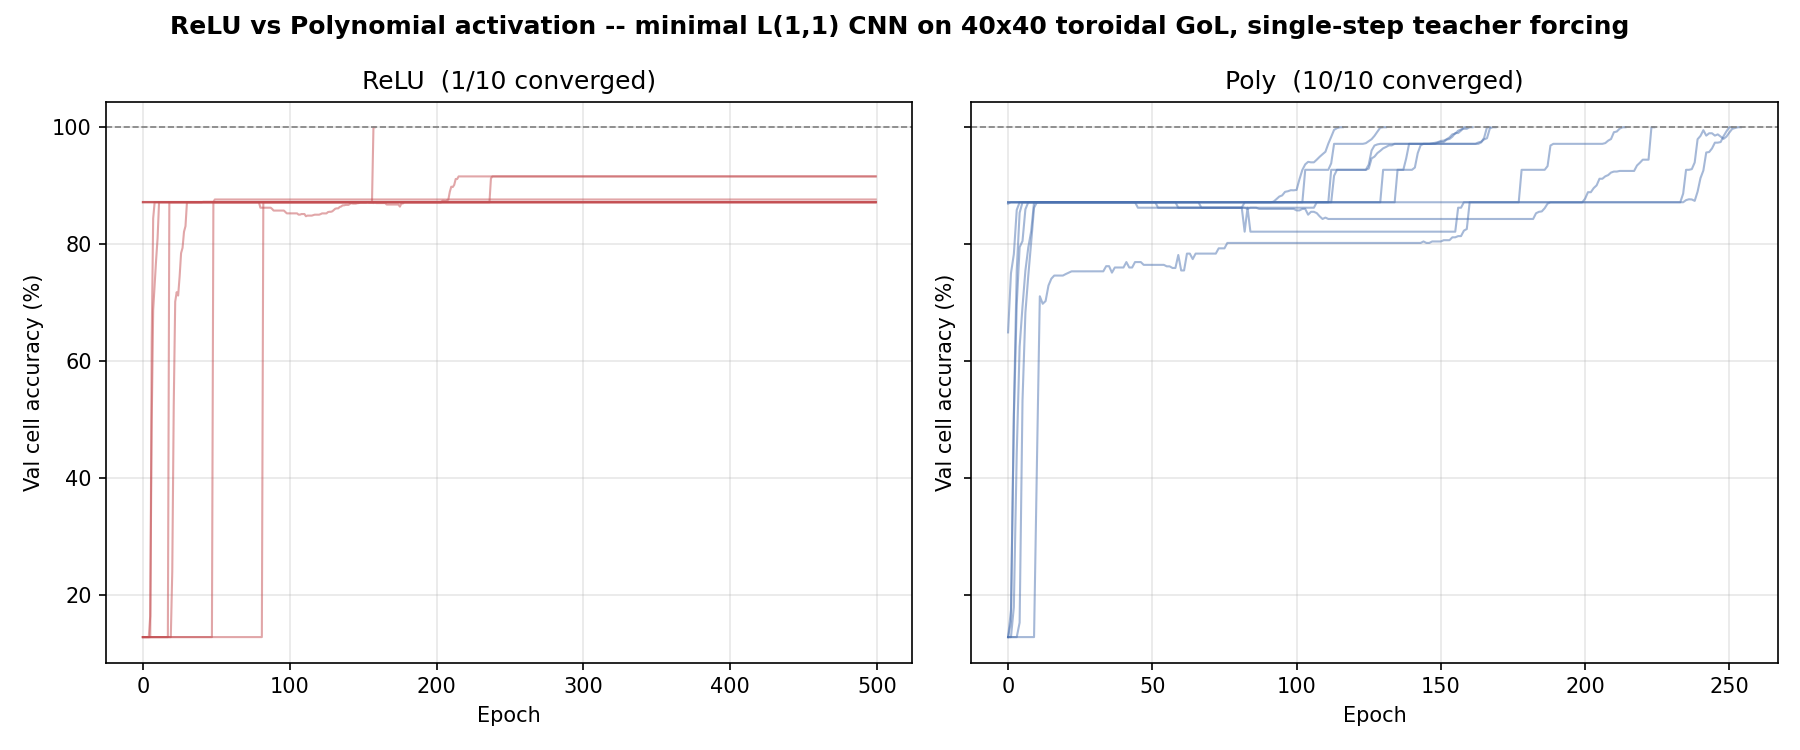
\includegraphics[width=0.9\textwidth]{figures/relu_vs_poly_convergence.png}
  \caption{Validation accuracy over training, all 10 seeds. ReLU (left)
  plateaus around 87--92\% for 9 of 10 seeds and never escapes; polynomial
  activation (right) reaches 100\% accuracy on every seed.}
  \label{fig:relu-vs-poly}
\end{figure}

The reproduction (Table~\ref{tab:relu-vs-poly}, Figure~\ref{fig:relu-vs-poly})
confirms the paper's claim under an independent implementation, a different
grid size, and a different (and much smaller) training set than the
original paper used: ReLU converges to perfect accuracy on only 1 of 10
seeds, plateauing at 87--92\% cell accuracy on the rest, while the
polynomial activation converges to perfect accuracy on all 10 seeds,
typically within 120--260 epochs (each run completing in 1--2 seconds on
CPU, given the network's tiny size).

\subsection{Negative result: transferring the polynomial activation to the multi-step model}
\label{sec:v11}

Given the clean reproduction in Section~\ref{sec:reproduction}, we attempted
to transfer the polynomial activation into the CNN feature-extraction stage
of the full CNN-Transformer architecture (Section~\ref{sec:architecture}),
at V8's parameter budget ($d_{\text{model}}=64$, 4 layers): replacing the
two GELU activations in Stage 1 with the same learnable
$\phi(x)=w_0+w_1x+w_2x^2$ used in Section~\ref{sec:reproduction}, while
leaving the Transformer encoder's GELU unchanged. This adds only $288$
parameters over the baseline V8 architecture ($292{,}176$ vs.\ $291{,}888$),
so any accuracy change can be attributed to the activation rather than to
capacity. The model was trained from scratch with the same scheduled
sampling recipe used for V10 (Section~\ref{sec:training-evolution}): $K=3$
unrolled steps, $p: 0 \to 1$ over training, learning rate $10^{-4}$.

Training was \emph{not} stable. By epoch 5, validation metrics were
promising (F1 $=0.89$, born-accuracy $86.8\%$, validation loss $0.227$) ---
already close to V8's converged performance after only 5 epochs from
scratch. However, by epoch 10 the model had regressed sharply (validation
loss $0.491$, F1 $0.39$), and by epoch 15 it had diverged further
(validation loss $1.045$, F1 $0.17$), while per-epoch wall-clock time grew
roughly five-fold over the same interval. Training loss remained flat
throughout ($\approx 0.21$) even as validation loss exploded, indicating
the divergence is specific to the clean single-step evaluation distribution
rather than a general optimization failure.

We hypothesize this reflects an interaction between the polynomial
activation and the multi-step scheduled-sampling training loop that is
absent from the single-step setup verified in
Section~\ref{sec:reproduction}: the $w_2 x^2$ term is unbounded and,
unlike a saturating activation such as GELU, has no mechanism to suppress
large intermediate activations. Once scheduled sampling begins feeding the
model's own (initially imperfect) predictions back as input to later
unrolled steps, any activation values that drift into a regime where the
quadratic term dominates are amplified rather than clipped, compounding
across the $K=3$ steps in a manner structurally similar to the STE failure
mode identified for V6 (Section~\ref{sec:training-evolution}). We did not
observe this instability in Section~\ref{sec:reproduction} because that
experiment uses pure single-step teacher forcing with no autoregressive
feedback loop.

This negative result was not pursued further within the scope of this
report; we record it here as we consider the failure mode informative in
its own right, and as a caution against assuming an inductive-bias fix
verified in a minimal single-step setting will transfer unmodified to a
larger multi-step training regime. Candidate fixes --- left to future work
--- include bounding the quadratic coefficient (e.g.\ a saturating variant
$\phi(x) = w_0 + w_1 x + w_2 x^2/(1+x^2)$), using a separate, smaller
learning rate for the polynomial coefficients, or first verifying
single-step (teacher-forcing-only) training at V8/V10 scale before
introducing scheduled sampling.

\section{Discussion and Conclusion}

Three broad lessons emerge from this study.

\textbf{Exposure bias is a first-order concern for autoregressive
cellular-automaton models, and its fix must be chosen carefully.} Teacher
forcing alone (V5) produces excellent single-step metrics that do not
predict rollout stability. The most direct-seeming fix for multi-step
training --- a straight-through estimator (V6) --- fails due to a
systematic directional gradient bias rather than an optimization-stability
issue, and is not rescued by gradient clipping or a lower learning rate.
Scheduled sampling (V7), which avoids passing gradients across unrolled
steps entirely, resolves the problem cleanly. This distinction --- between
instabilities caused by gradient \emph{magnitude} and those caused by
gradient \emph{direction} --- recurred later in the polynomial-activation
negative result (Section~\ref{sec:v11}), where we again observed a
divergence with a similar signature (stable training loss, exploding
validation loss) under a different mechanism (an unbounded activation
interacting with autoregressive feedback rather than an STE gradient path).

\textbf{Aggregate validation metrics can hide severe, structured
regressions.} The V8-to-V9 comparison (Section~\ref{sec:training-evolution})
is the clearest demonstration: V9's validation loss and precision/recall
are statistically indistinguishable from V8's, yet its per-grid error count
at high density is an order of magnitude worse. This was only detectable
via a targeted, density-stratified failure search --- a general reminder
that i.i.d.\ validation splits can fail to surface regressions concentrated
in identifiable input subpopulations, and that practitioners should audit
per-subgroup behavior rather than relying on a single scalar validation
metric, especially before deciding that a change (like scaling up training
data) has helped.

\textbf{Once a model is capacity-limited, only capacity fixes the problem.}
The clearest evidence for this is negative: V9 attempted to resolve V8's
residual high-density errors purely with more data (of a kind the model
already saw extensively) and made things worse. V10 held the data
distribution fixed and scaled the model 5.15$\times$, and eliminated all
2,500 evaluated per-grid errors. This is consistent with, though not
identical to, the picture in Ahmed \& Davis \cite{ahmed2026polynomial}: they
show that a poorly-matched inductive bias (ReLU) can make a
network fail to learn a rule it is representationally capable of encoding
with very few parameters, while we show that once a specific
\emph{well-matched} architecture (GELU CNN-Transformer with scheduled
sampling) has saturated its capacity at a given width, adding width is what
resolves the remaining gap --- not more data of the same kind. Our
attempt to combine both ideas (Section~\ref{sec:v11}) was unsuccessful in
its first iteration, underscoring that these two levers do not necessarily
compose for free, particularly once autoregressive training is involved.

\textbf{The embedding analysis (Section~\ref{sec:embedding-analysis})}
provides a mechanistic complement to the accuracy results: it shows
directly, via patch-level cosine similarity and PCA projections, that the
model's learned absolute positional embedding is responsible for most of
its sensitivity to geometric transformations on dense grids, while sparse
configurations are nearly embedding-invariant simply because most patches
are empty on both sides of any transformation. This is consistent with the
architectural choice (Section~\ref{sec:architecture}) to augment with the
dihedral group $D_4$ but not with translation, since translation
augmentation would directly conflict with a learnable absolute positional
embedding.

\subsection*{Limitations and future work}

This report reflects a single training run per configuration for the
CNN-Transformer experiments (V5--V11), aside from the deliberately
multi-seed reproduction in Section~\ref{sec:reproduction}; conclusions
about V6/V9/V11 instability would be strengthened by repeating those runs
across seeds, as we did for the minimal-CNN verification. The V11 negative
result (Section~\ref{sec:v11}) was not root-caused beyond the hypothesis
offered; a natural next step is to test the polynomial activation in a
single-step-only (teacher-forcing) training regime at V8/V10 model scale,
isolating whether the instability is intrinsic to the activation at this
model size or specific to its interaction with scheduled sampling. The
per-grid failure-search protocol used throughout
(Section~\ref{sec:training-evolution}) covers five densities and a small
set of named patterns; a more exhaustive audit (finer density grid,
targeted adversarial search) might reveal further tail-case regressions
not captured here, including for V10 despite its zero-error result on the
2,500 grids tested.


\bibliographystyle{plain}
\bibliography{references}

\end{document}
